% !TEX root = ../notes_template.tex
\chapter{Micro-Circulation}\label{chp:ecf_microcirculation}
Updated on \today
\minitoc

The ECF supports muscle fibers by having the correct resources necessary for muscle function. ECF resources include the correct concentration of ions, the availability of nutrients and molecules such as oxygen. The ECF is also where things moved from the muscles end up until they can be metabolized or removed from the body. Exchange between the ECF and intra-cellular fluid (ICF) is selective for ions, molecules and nutrients but comparatively free for water. The function of muscle fibers depends on the homeostasis of ECF oxygen, carbon dioxide, sodium, potassium, calcium, water, pH, and temperature.
The micro-circulation supports the ECF. Micro-circulation ensures a continuous circulation of the ECF between its two compartments, vascular and interstitial. Water, ions, molecules and nutrients are constantly circulating between the vascular (capillaries and lymphatics) and interstitial compartments of the ECF. 

% 

\vspace{5mm}

\textbf{Objectives include:}
\begin{enumerate}
    \item Explain the basic dependency of muscle fibers on the extra-cellular fluid.
    \item Explain the basic dependency of extra-cellular fluid on the micro-circulation, circulation, renal filtration, respiration, ventilation, digestion, absorption, metabolism and elimination.
    \item Explain the difference between vascular, interstitial and intra cellular fluid.
    \item Explain the role osmosis, osmolarity and osmotic pressure play in micro circulation between ECF-ICF and various situations leading to intra-cellular edema.
    \item Explain the components, roles and implications of the parameters of the filtration equation to explain net filtration and filtration at each end of the capillary.
    \item Use the filtration equation to explain various causes of extra-cellular edema.
    \item Compare and contrast smooth muscle and skeletal muscle.
    \item Explain the underlying mechanism for the effectiveness of compression in edema management.
\end{enumerate}

\section{Muscle Support Overview}

The chapters of Part II are about the supportive environment of the ECF. Every chapter describes a set of functions that serve the purpose of delivering, removing or regulating the contents of the ECF. This chapter focuses on the process of micro circulation of water and filtration of ions, molecules, nutrients and heat between the  vascular compartment of the ECF and the interstitial compartment, the non vascular compartment of the ECF.  

% Type something

Figure \ref{fig:part2_overview} is a graphic representation of the chapters of Part II. Filtration relies on micro-circulation which relies on circulation. Circulation is the flow of blood through the entire circulatory system, covered in Chapter \ref{chp:circulation} on Blood Flow. Circulation of blood through the entire body ensures regular mixing of the ECF contents throughout the body. This mixing ensures consistency of ECF contents and a stable environment for all the cells of the body. For example, if blood $Na^+$ concentration is tested, it is properly assumed that concentration is the concentration of $Na^+$ throughout the entire ECF. Circulation also allows that each supporting system contribute - either to adding water, heat, ions, molecules or nutrients to the ECF, or removing by-products from the ECF. Supporting systems are also in communication with one another based on the circulating substances and messages (hormones). For example, if a muscle working at high tension is shuttling lactate into the ECF, it is picked up by the circulation and can then enter other cells (heart, liver, non working muscles) where lactate levels are low. In these cells the lactate can be used to produce an $NADH$ from $NAD^+$, and a pyruvate to proceed into the mitochondria. The circulation is the nationwide transportation and distribution system that gets a package from the local post office to a post office across the country. The micro circulation is the delivery from the local post office to and from a mailbox at an address.

The contents of blood is regulated and supported by renal filtration (kidneys) and endocrine system, covered in Chapter \ref{chp:blood_content} on Blood Volume. The regular circulation of blood through the kidneys involves several mechanisms that selectively filter the blood and in doing so regulate the ECF, and therefore the ICF volume. The regulation of fluid volume includes the regulation of several important ions (electrolytes) and the removal of waste (i.e. urea). Working with the endocrine system the kidneys provide long term regulation of blood pressure, which is important for circulation; as well as red blood cells, which is important for oxygen carrying capacity.

Cellular respiration in the mitochondria is constantly using $O_2$ and producing $CO_2$. These molecules are called gases (blood, alveolar) because their natural state is in the gaseous form. The micro circulation ensures the regular delivery ($O_2)$ and removal ($CO_2$) of these gases from the interstitial fluid. The circulation to the lungs ensures the regular exchanges of these gases with the environment. Blood gases rely on blood flow through the lungs for respiration (gas exchange) between the blood and alveoli, covered in Chapter \ref{chp:blood_oxygen} on Blood Gas. Respiration depends on ventilation, the regular movement of these gases into and out of the lungs with the bulk transport of air. Ventilation is covered in \ref{chp:alveolar_oxygen} on Alveolar Gas. 

Maintaining blood nutrients relies on digestion, absorption, metabolism and elimination by the gastrointestinal organs and the liver. Based on the basic physiological concept of mass balance the regular elimination of water requires the regular intake of water. The regular transformation of the carbon bond energy from carbohydrates and fats requires the regular intake of carbohydrates and fat. The regular use, breakdown and elimination of proteins for cellular functions requires the regular intake of protein. All together these processes are covered in Chapter \ref{chp:blood_nutrients} on Visceral Support.

\begin{figure}[!h]
    \centering
    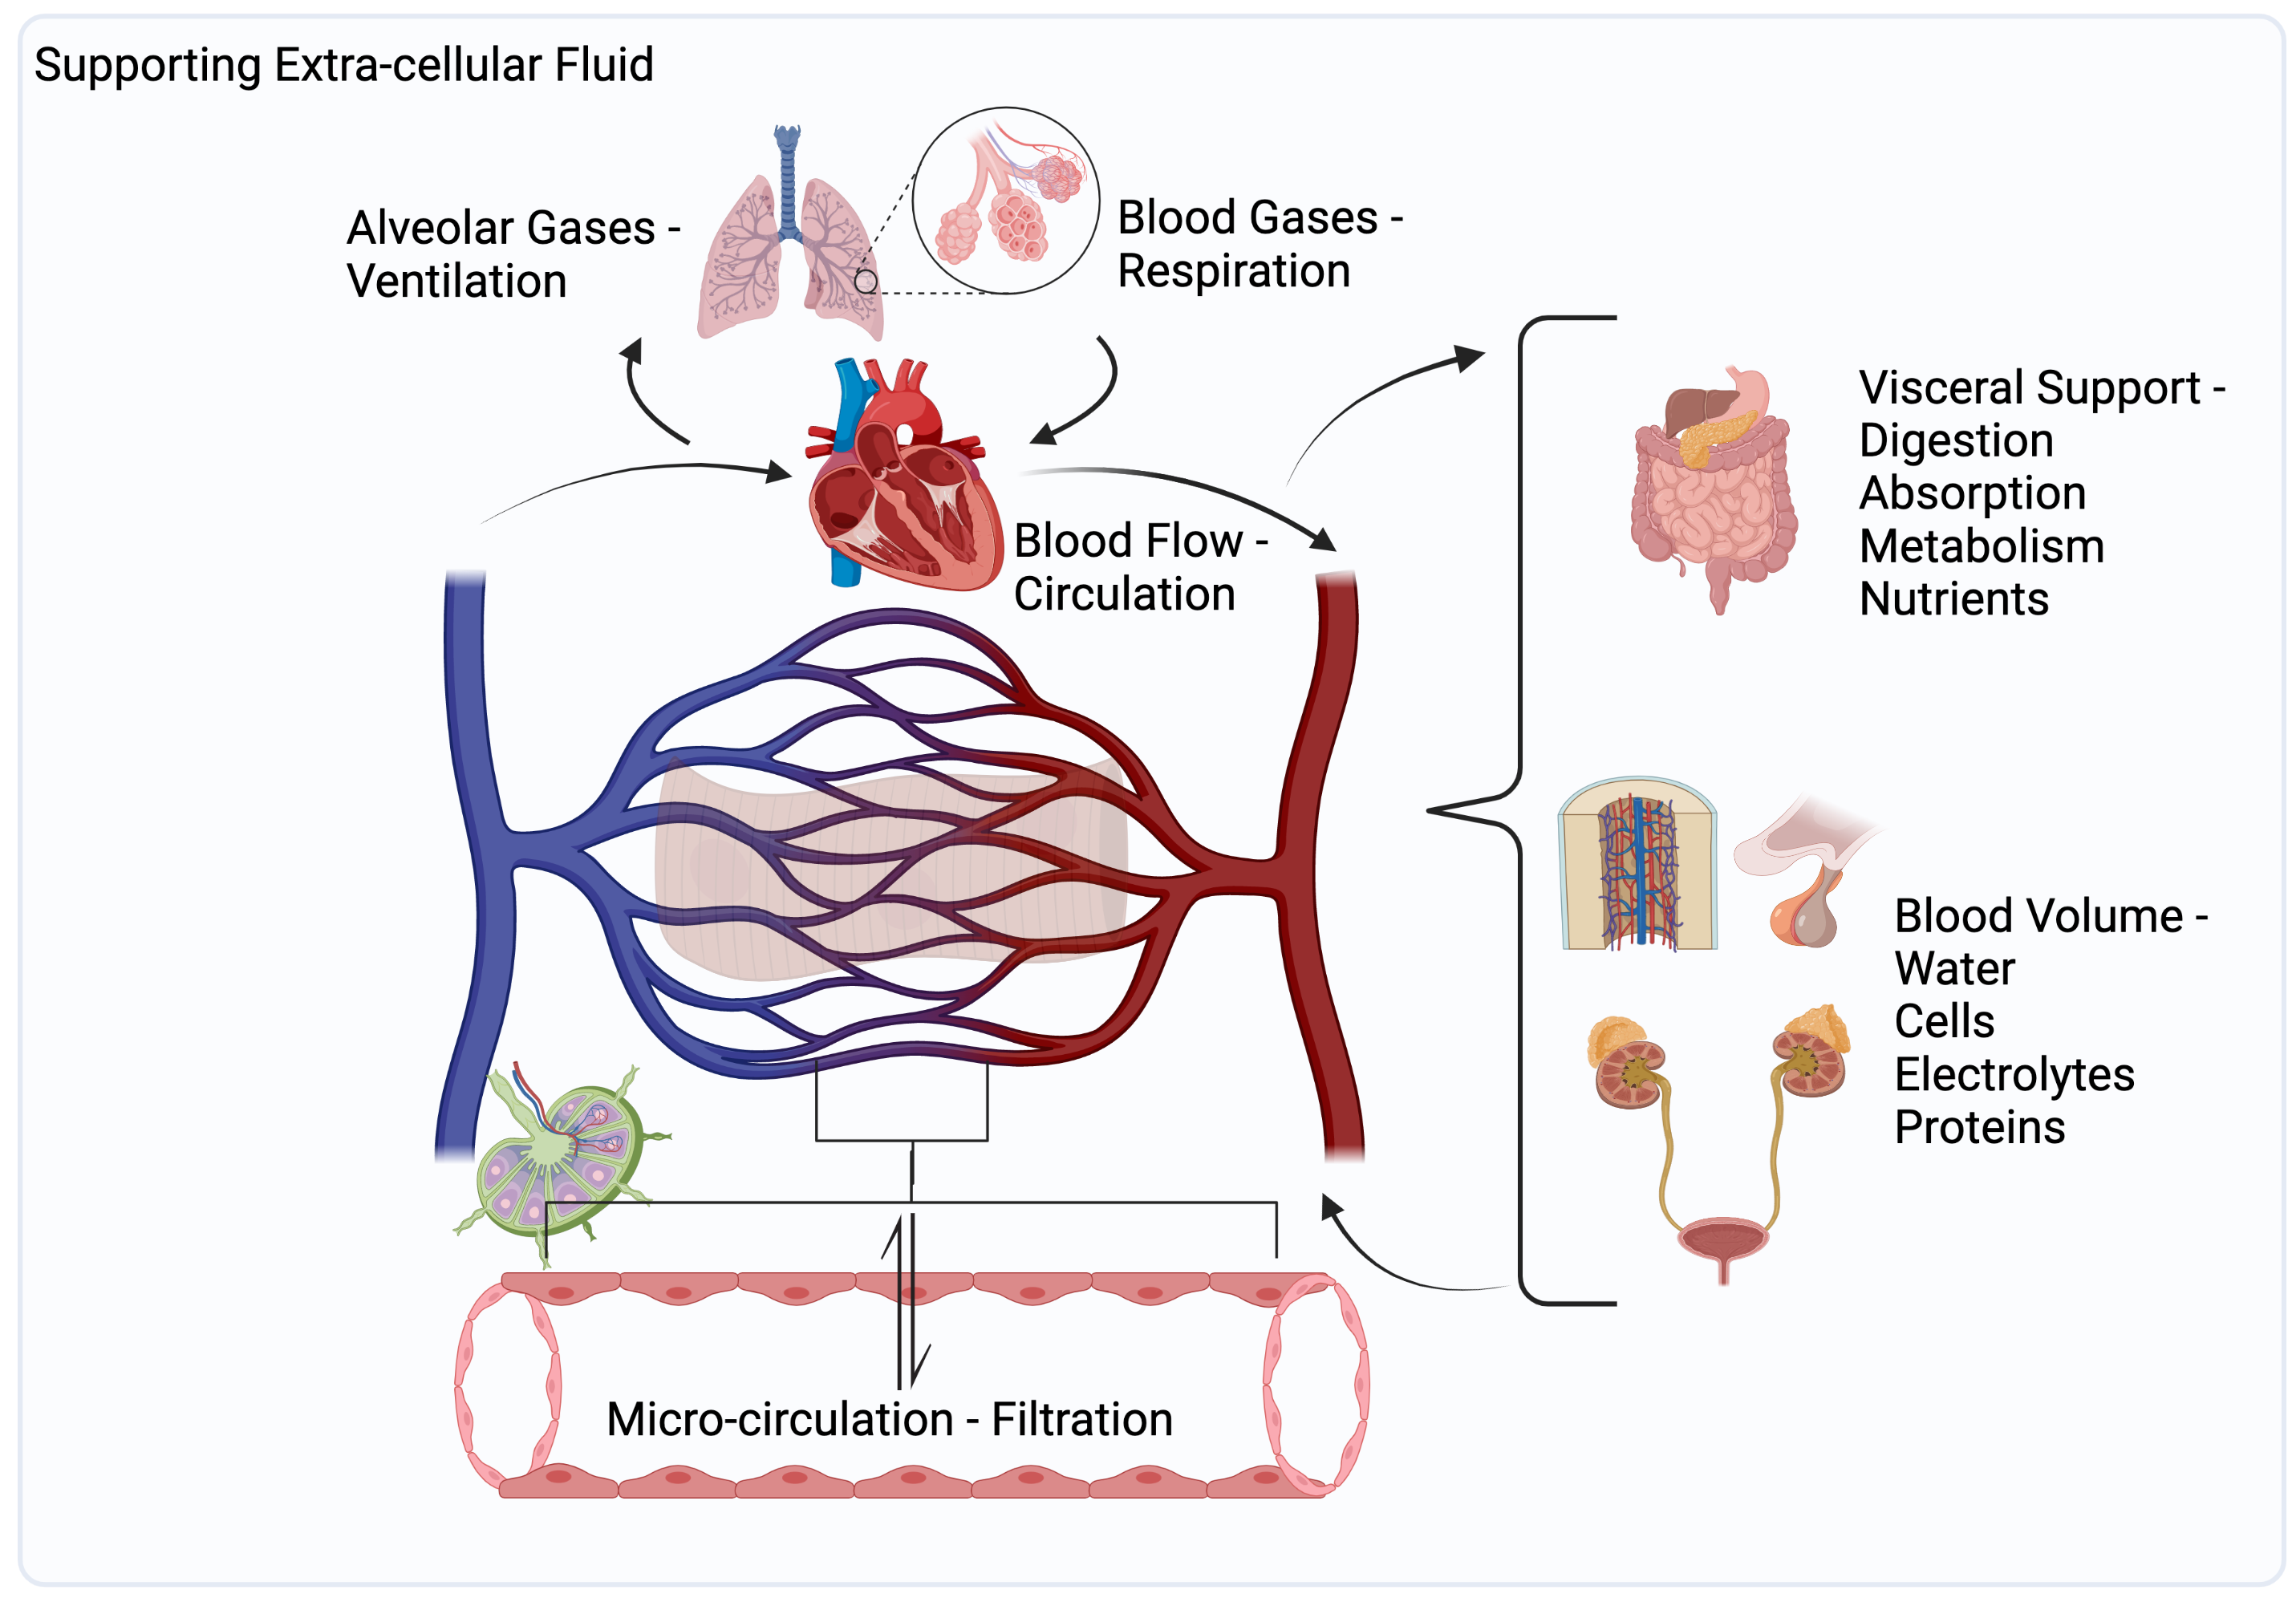
\includegraphics[width=1\linewidth]{./figure/part2_overview.png}
    \caption{Part II: Muscle Support Overview \footnotesize{Created with BioRender.com}}
    \label{fig:part2_overview}
\end{figure}

Together these systems support the ECF and therefore muscle fibers and muscle function. They maintain homeostasis of several important electrolytes (ions, including $H^+$ as measured by pH), nutrients, molecules, water and heat (temperature). The systems are are integrated with several interactions and redundancies to provide support across a wide range of muscle demands in a wide range of circumstances, both good and bad.

One difference between Part I and Part II of the book is that many topics throughout the chapters are in Part II are inherently \textit{Clinical Physiology Connections}. Since the concepts described in Part II are traditional concepts in a clinical physiology course, in many ways these chapters are, in their entirety, clinical physiology connections. As the occasion arises, in pace of \textit{Clinical Physiology Connections} there will be \textit{Muscle Connections} as in this chapter on Smooth Muscle.

\section{Micro Circulation}

Micro-circulation is the continuous movement of ions, nutrients and molecules between the blood plasma (vascular part of ECF) and interstitial fluid. Micro-circulation occurs through the semi permeable capillary membranes in a process called filtration. The capillary membranes allow relatively free passage of water, ions, molecules and  nutrients (other than proteins). The contents of plasma and interstitial fluid is similar other than cell and protein content (particularly red blood cells and albumin), due to an inability of these larger items to pass through the capillary membrane. There are also differences in $O_2$ and $CO_2$ due to the constant exchange with the cell.

Normal values of several important ions, molecules and nutrients are depicted in Figure \ref{fig:ecf}. Vascular and interstitial values are typically equal unless otherwise noted. $O_2$ and $CO_2$ pass easily through both the semipermeable capillary membrane and the semipermeable sarcolemma. There is a relatively large gradient for these molecules that varies due to the muscle fiber energetics. Normal function of circulation, respiration and ventilation at sea level are capable of equilibrating the vascular $O_2$ and $CO_2$ content even extreme high energetic situations.

\begin{figure}[!h]
    \centering
    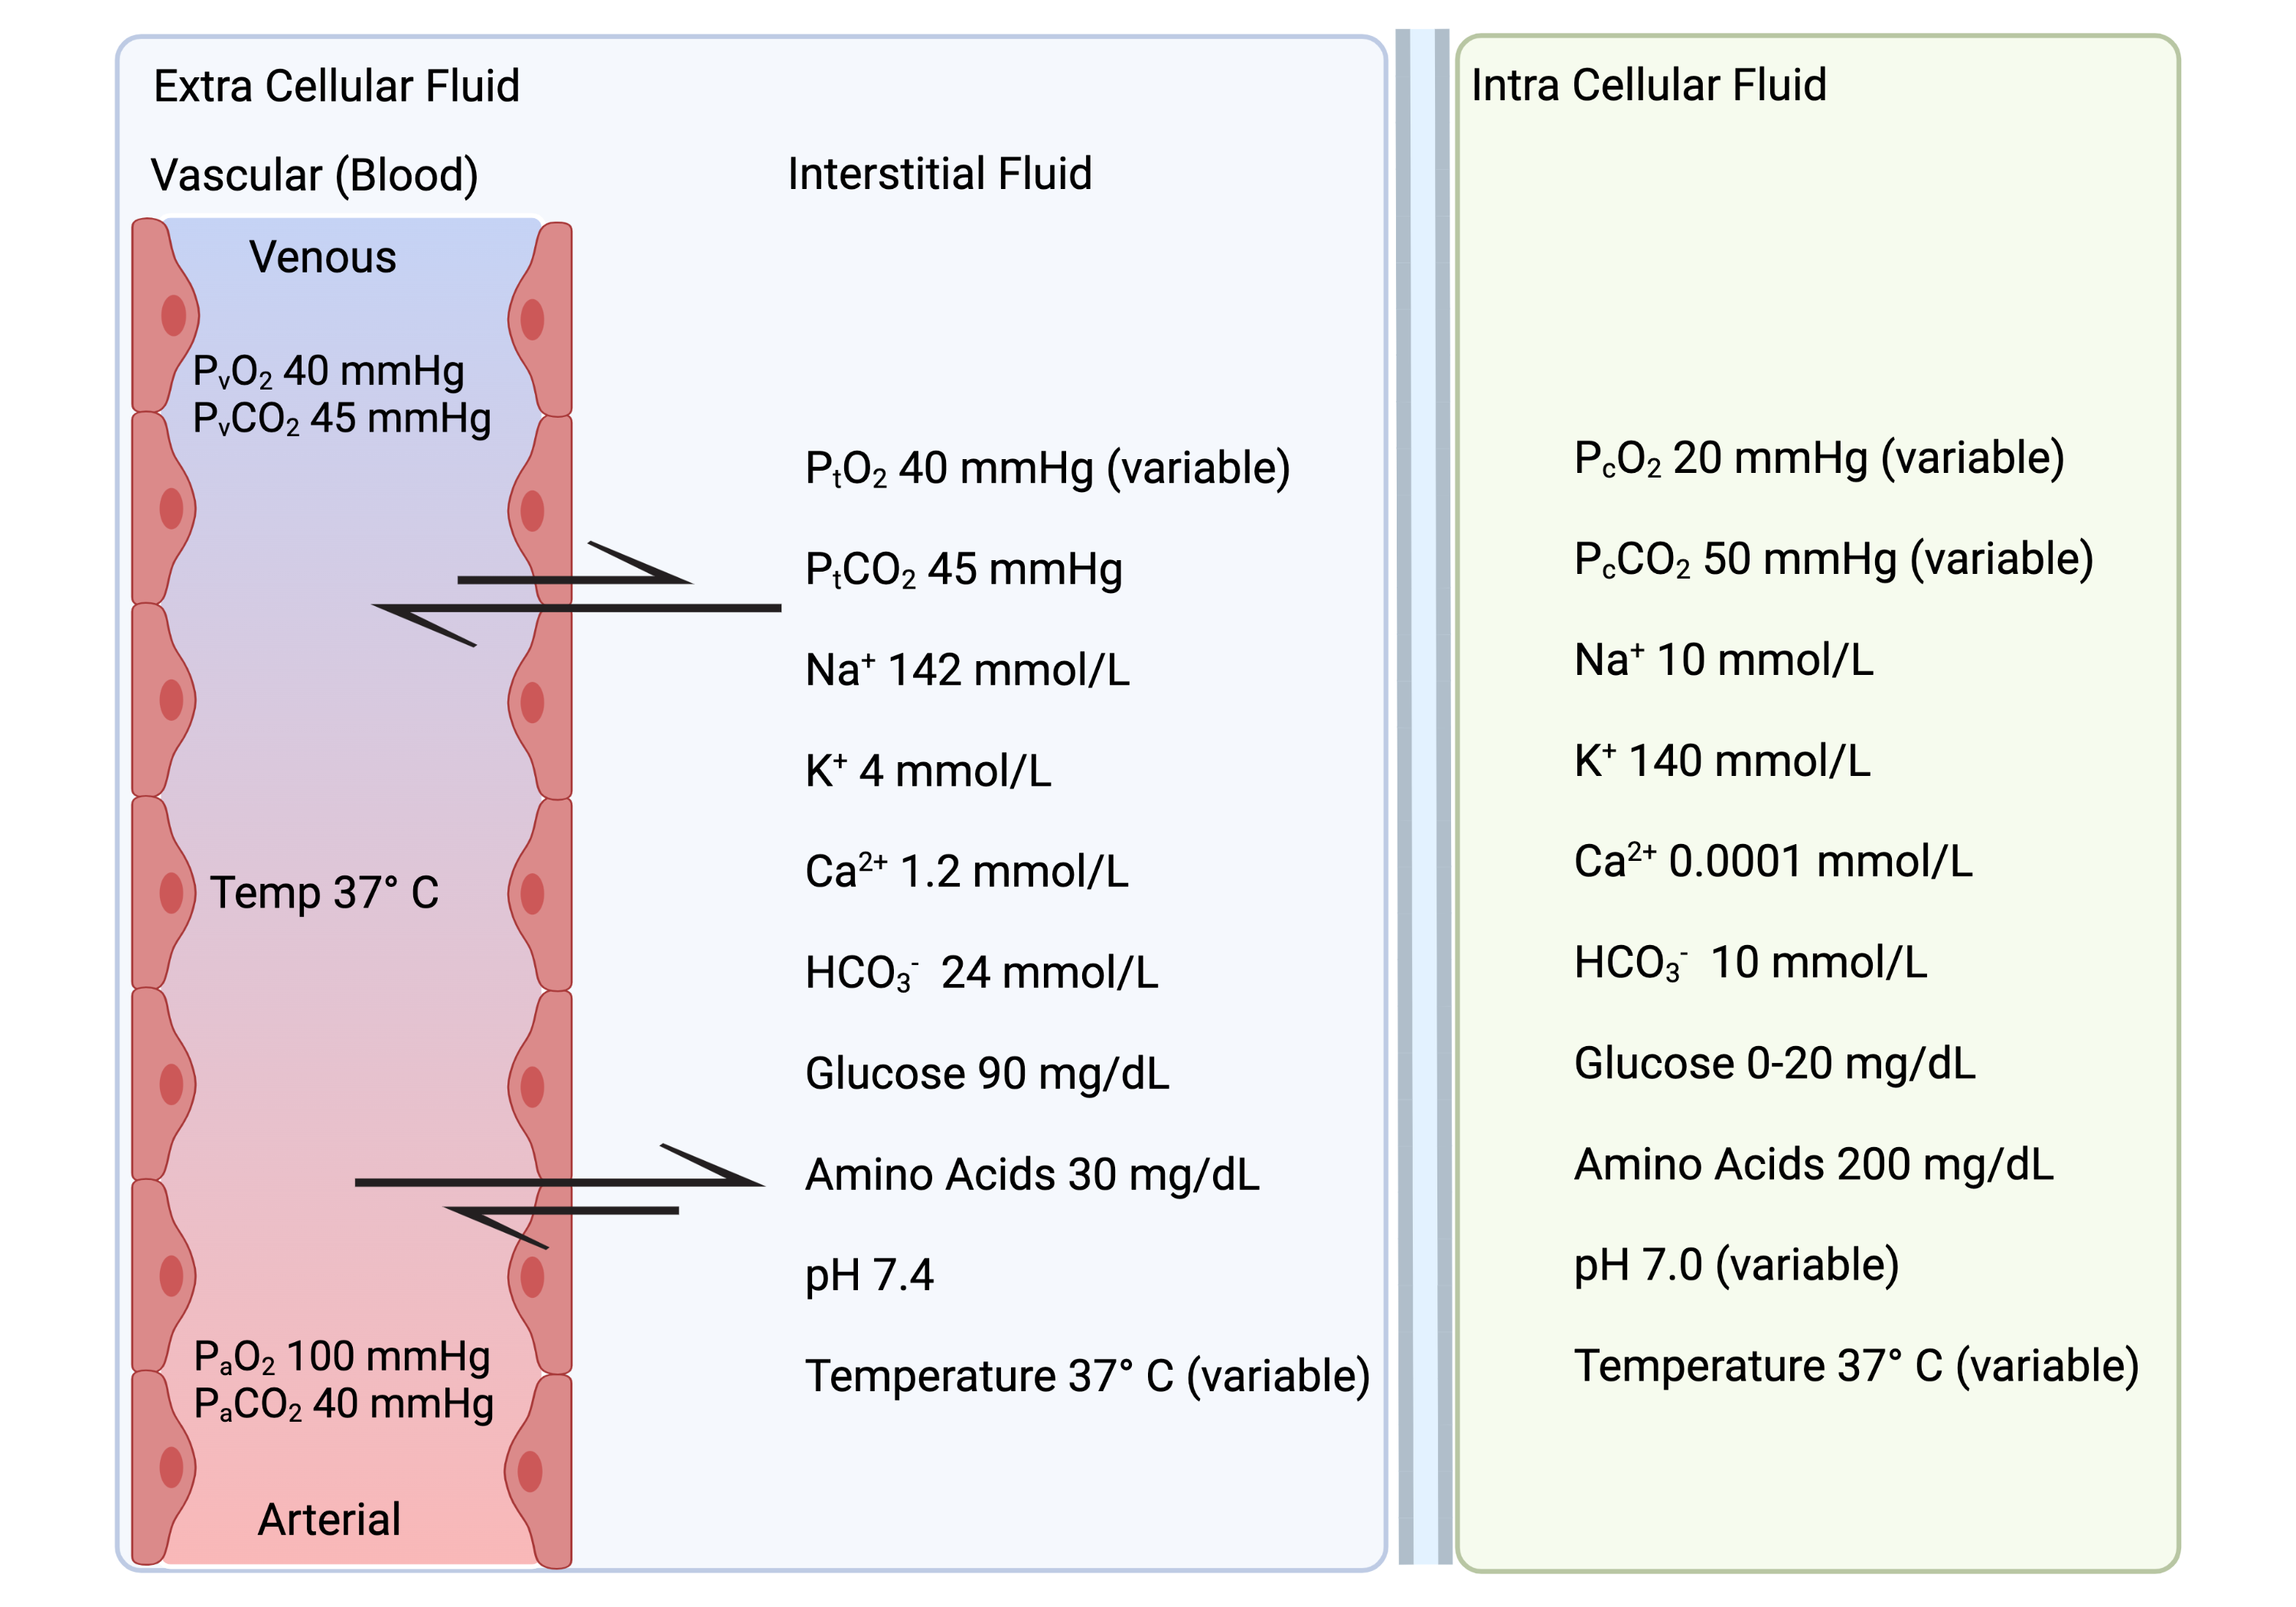
\includegraphics[width=1.0\linewidth]{./figure/ecf.png}
    \caption{Extra-cellular (Vascular \& Interstitial) and Intra-cellular Fluid \footnotesize{Created with BioRender.com}}
    \label{fig:ecf}
\end{figure}

\subsection{Extra Cellular - Intra Cellular Fluid Movement}

Exchange between the interstitial fluid and intracellular fluid occurs through the semi permeable cell membrane (sarcolemma). The sarcolemma restricts movements of ions and even with changes in the permeability for $Na^+$ and $K^+$ during excitation does not change the concentration difference between the interstitial and ICF fluid for these ions (at least under normal circumstances). The sarcolemma regulates the movement of nutrients.  Glucose uptake by a cell is influenced by the activation of the glut4 receptor channel for glucose by insulin. 

Between 50-70\% of an adult body is water. The variation in the percent of the adult body that is water is based on variations in lean (mostly muscle) tissue. In individuals with more muscle (compared to adipose tissue) there is a higher percent of water. Of the total body water approximately 2/3 is intracellular (ICF) and 1/3 is extra cellular (ECF). Since water moves freely between the interstitial and ICF due to a large quantity of aquaporins (water channels) in the cell membrane the balance of ICF and ECF water volume is based largely on solute concentrations and resultant balance of osmotic pressure.

\subsubsection{ECF - ICF Water Volume Balance}

The sarcolemma is permeable to water but not to the ions. The osmolarity between the ECF and ICF determines whether there is net water movement by osmosis and the water (fluid) volume shifts between ECF and ICF. Under steady state conditions the osmolarity between the ECF and ICF is equal. Changes in solute concentration (ions, molecules, nutrients) in the ECF and ICF changes the osmolarity and results in movement of water until osmolarity balance is achieved.

\paragraph{Review of Osmotic Pressure}

At this point most people benefit from a review of these terms and the associated process of osmosis and osmotic pressure. Osmosis is the net movement of water across a selectively permeable membrane caused by a concentration difference across the membrane. Osmotic pressure is the pressure required to prevent osmosis of water through a membrane that is permeable to water but not to the solute (similar concept to an equilibrium potential). The osmotic pressure is an indication of how quickly osmosis occurs (driving force); and osmosis does not occur if there is no osmotic pressure gradient. Osmotic pressure is exerted by particles and is determined by the number of particles per unit volume of fluid. 

The osmole (Osm) expresses solute concentration in terms of the number of particles. An Osm is the number of moles of solute that contribute to the osmotic pressure of a solution. Osmolarity refers to the number of osmoles in a volume (Liter (L)) of solvent. Osmolarlity = Osm / L. Osmolarity is proportional to the milli osmoles / L as well (mOsm/L).

Osmotic pressure ($\pi$) is directly proportional osmolarity (concentration in Osm in a volume (L) of solvent) ($C$); the ideal gas constant ($R$); and absolute temperature ($K = 310^{\circ}$ at body temperature) in the equation: $\pi = C \cdot R \cdot T$. Since $R$ is a constant, and $K$ in the body varies within a relatively narrow boundary, the osmotic pressure is determined by the osmolarity (Osm/L). At body temperature each 1 mOsm/L (milli osmole per liter) results in approximately 19.3 mmHg of osmotic pressure. In Figure \ref{fig:osmotic_pressure} the solution on the left has 1 mOsm/L more osmolarity. At body temperature this means 19.3 mmHg of pressure is required to stop the movement of water. Differences in osmolarity due to differences in solute concentration across the sarcolemma results in osmosis of water until there are no differences in osmolarity.

\begin{figure}[!h]
    \centering
    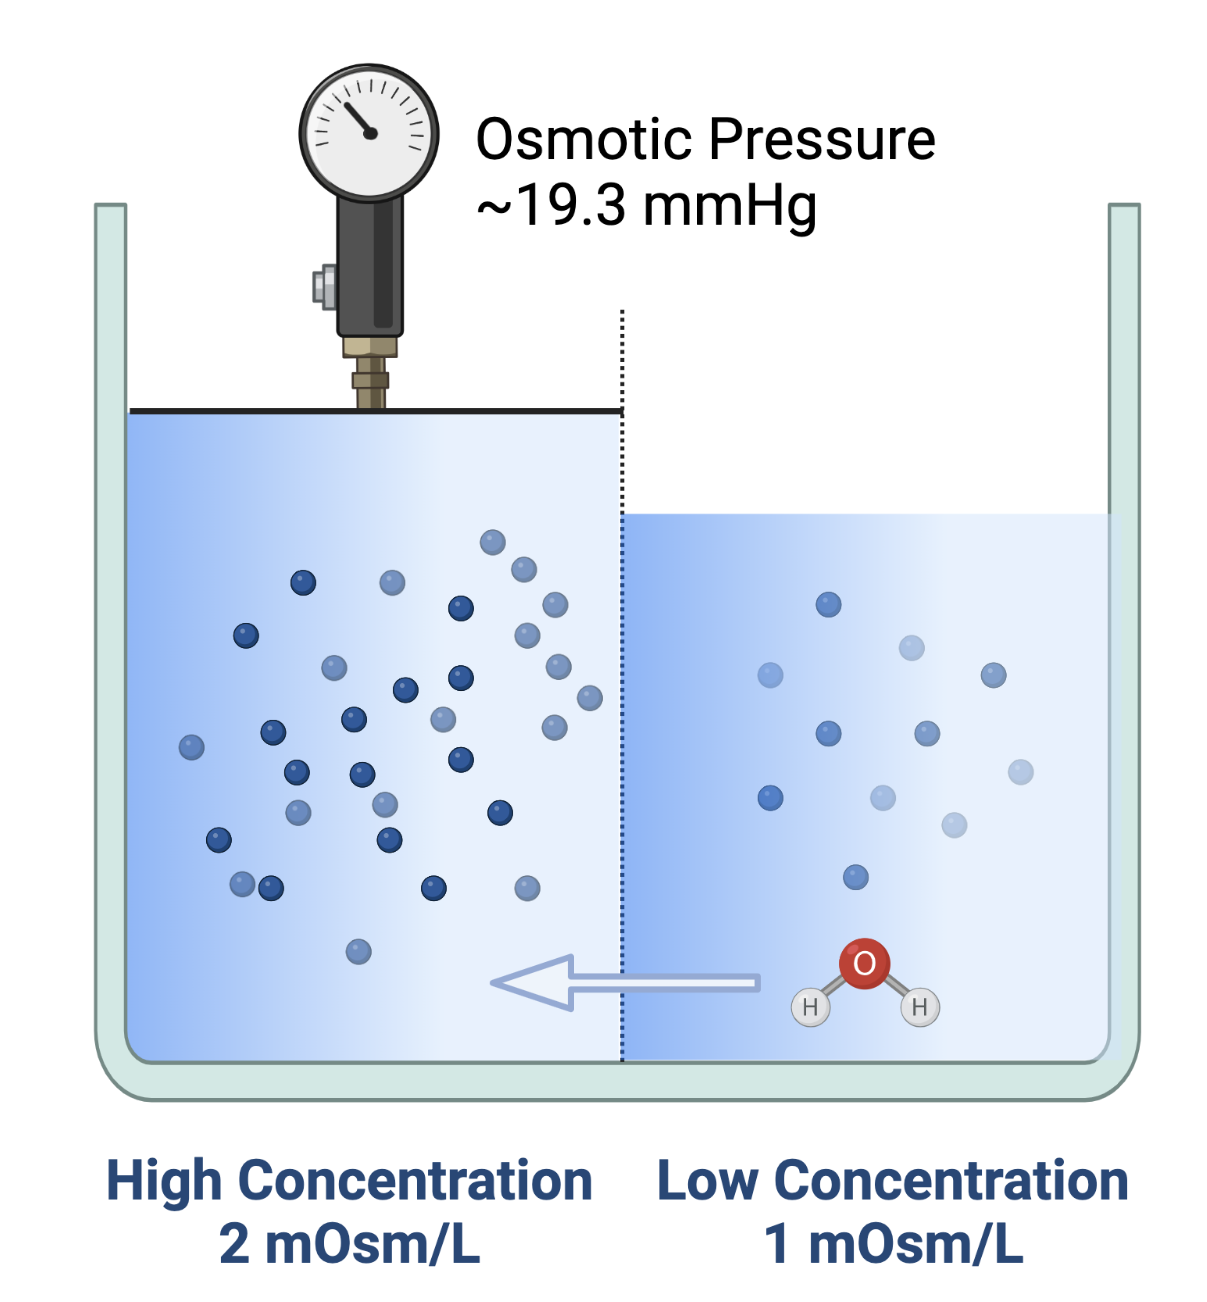
\includegraphics[width=0.5\linewidth]{./figure/osmotic_pressure.png}
    \caption{Osmotic Pressure \footnotesize{(Created with BioRender.com)}}
    \label{fig:osmotic_pressure}
\end{figure}

Since water moves freely across the sarcolemma osmosis occurs and balances the osmolarity of the ICF with that of the ECF. When the osmolarity of ECF and ICF are equal there is no osmosis or net movement of water across the membrane since the osmotic pressures cancel each other out.

The total intake of water and ions (electrolytes) are carefully matched by equal outputs from the body to prevent fluid volumes and ion concentrations from fluctuating beyond acceptable ranges (mass balance, and homeostasis). There are times when there are differences between intake and output of water and ions that eventually must be remedied. Small shifts in water between ECF and ICF ensure that both compartments have the water required and maintain appropriate ion concentrations.

These shifts typically start with changes to the ECF. It is usually the ECF that we are adding, or removing, water and ions to, or from, (ingestion, absorption, renal filtration). Water and ions are also removed from ECF in the kidneys, the colon (small amount under normal circumstances) and water is removed from ventilation.  These changes in water volume change the concentration and therefore osmolarity of ECF. 

% All things that enter the ICF do so from the ECF, the ICF does not typically have changes to osmolarity that are not provoked by the ECF first. There are some circumstances discussed below that ICF osmolarity may change in response to abnormalities in ICF $K^+$ concentration. 

The response to changes in osmolarity between the ECF and ICF is movement of water by osmosis until there is once again equalize the osmolarity. Large water intakes to the ECF such as large water intake or IV infusions; or decreases (dehydration) associated with sweating, GI fluid loss, or excessive urine formation by the kidneys (i.e. in diabetes mellitus) change the ECF water volume. If these changes alter the osmolarity of the ECF then water will pass between ECF and ICF until osmolarity is equalized.

Figure \ref{fig:iso_hypo_hypertonic} depicts the changes that would occur to the osmolarity with the addition of a volume of isotonic (same osmolarity), hypotonic (lower osmolarity), and hypertonic (higher osmolarity) solution to the ECF.

\begin{figure}[!h]
    \centering
    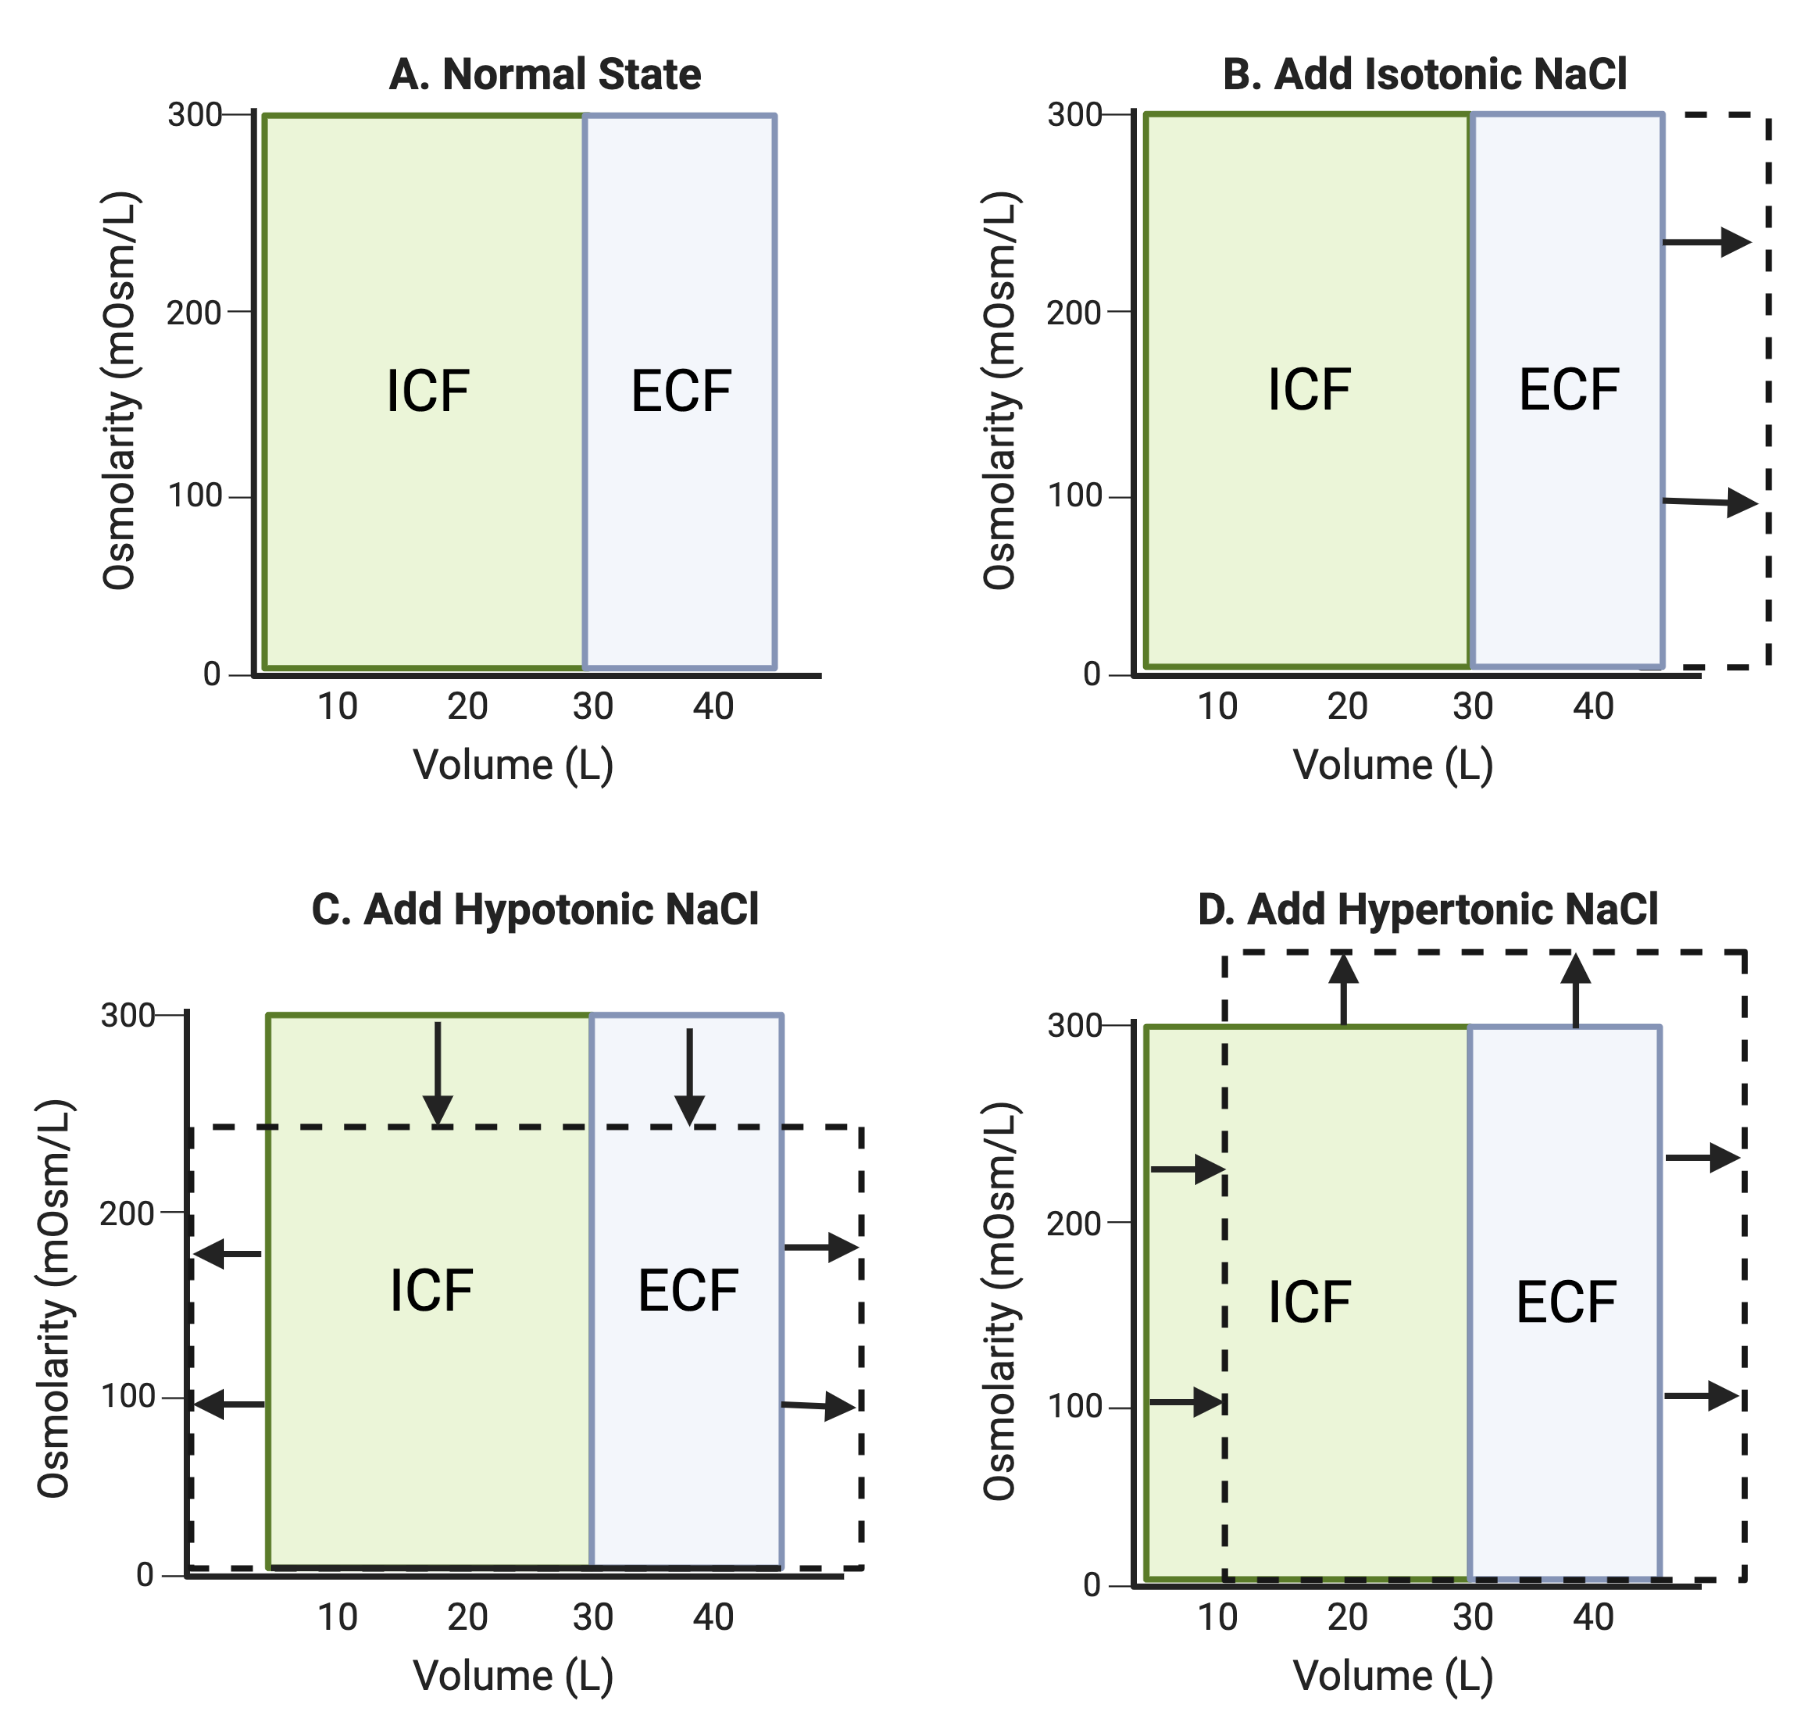
\includegraphics[width=0.7\linewidth]{./figure/iso_hypo_hypertonic.png}
    \caption{Impact of ECF Infusions of Iso, Hypo and Hypertonic Solutions (See text for details) \footnotesize{(Created with BioRender.com)}}
    \label{fig:iso_hypo_hypertonic}
\end{figure}


\begin{itemize}
    \item Adding an isotonic solution to ECF does not change osmolarity of the ECF so there is no osmosis (no change in net water movement). The end result is an increase in ECF volume but no change to ICF volume (See Figure \ref{fig:iso_hypo_hypertonic} B).
    \item Adding a hypotonic solution to ECF decreases the osmolarity of ECF and results in osmosis of water into the cells (ICF) and increases ICF volume. This continues until the osmolarity of ICF decreases and the concentration of ECF increases until the osmolarity of both compartments are equal which stops the net flow of water into the ICF. The overall effect is increased ICF and ECF volume, and decreased ICF and ECF osmolarity (See Figure \ref{fig:iso_hypo_hypertonic} C). 
    \item Adding a hypertonic solution to ECF increases the osmolarity of ECF and results in osmosis of water out of the cells (ICF) and decreases ICF volume. This continues until the osmolarity of ICF increases and osmolarity of both compartments are equal which stops the net flow of water out of the ICF. The overall effect is decreased ICF volume and increased ECF volume; and an increase of osmolarity of both ICF and ECF See Figure \ref{fig:iso_hypo_hypertonic} D).
\end{itemize}

\paragraph{Importance of Osmosis to Muscle Excitation}

Changes in the osmolarity of the ECF and ICF are based on the concentration of these solutions. The concentration changes with changes to the water volume or changes to the amount of solute. A hypertonic solution therefore increases the concentration of $Na^+$ in both the ECF and ICF, but retains the concentration gradient. A hypotonic solution decreases the concentration of $Na^+$ in the ECF and ICF, but does not change the concentration gradient. Since the concentration gradient of $Na^+$ (and all ions) across the sarcolemma is critical to excitation, it should be clear that these osmotic pressure directed fluctuations to water volume serve an important buffer capacity to maintain these ion concentration gradients. Dehydration, a reduction in water volume, ultimately results in a slightly higher concentration of ions, but this higher concentration is balanced between the ECF and the ICF, so gradients are kept constant.
Ion abnormalities exist (electrolyte imbalances), but they do not have as profound an impact as they would if water did not move freely between ECF and ICF to normalize concentration gradients. 

\paragraph{Intra Cellular Edema}

Intra cellular edema is when there is increased fluid in the intra cellular space. Edema of the ICF can occur locally or systemically. As described above, ICF edema can occur with the addition of a hypotonic solution to the ECF (See Figure \ref{fig:iso_hypo_hypertonic} C). In general, any situation that reduces the osmolarity of the ECF can result in ICF edema. Hyponatremia (low ECF $Na^+$) reduces the ECF osmolarity, which results in a fluid shift from ECF into the ICF until the osmolarity between these compartment equalizes. This is an example of systemic ICF edema (effects all cells). Since this fluid shift from ECF to ICF is systemic it tends to be self limiting - the osmolarity between the ECF and ICF will eventually reach a balance.

Local depression of energetic systems which can occur due to a lack of adequate nutrition or $O_2$ (i.e. hypoxia) can increase the osmolarity of the cells and pull more water (locally) in from the ECF. In this situation there are two contributing problems. First, is a local depression of the $Na^+/K^+$-ATPase pumps (for lack of ATP) which leads to an accumulation of $Na^+$ inside the cell. Second, the accumulation of lactate and $H^+$ in the cell cannot be balanced by the removal. Keep in mind, this situation entails depression of energetic systems due to a lack of oxygen. If that lack of oxygen cannot be remedied with a reduction in ATP demand then the imbalance will persist until the cell dies. Cell death occurs when the cell membrane is no longer intact. The above scenario includes an acid pH (damaging to the cell membrane) and cellular edema (damaging to the cell membrane). The increase in cellular osmolarity (since it is a local occurrence) does not (or cannot) lead to a balance of osmolarity between the ECF and ICF because it is not systemic. The local cells cannot pull in enough fluid to alter the osmolarity of the entire ECF.

Extracellular edema can also cause intracellular edema if the extra cellular edema lowers the ECF osmolarity. Similar to adding a hypotonic solution to the ECF or in the case above of hyponatremia, with reduced ECF osmolarity the ICF osmolarity would pull water into cells until the osmolarity is equalized. A hypotonic solution is water (isotonic is water with 0.9\% NaCl or 5\% glucose). Adding too much water to the ECF (over drinking water) before adequate renal filtration and secretion can occur can lead to extra cellular edema and reduced ECF osmolarity. Note, problems with renal filtration and secretion (i.e. kidney failure) does not create this problem because there is also a build up of urea and other solutes in the ECF. So kidney failure does not cause a reduction in osmolarity of the ECF, but might cause an increase in the osmolarity of the ECF. 

\subsection{Extra cellular Values \& Ranges}

Table \ref{table:ecf_value_ranges} provides normal values and ranges and non lethal limits for several important components of the ECF.  The wide normal ranges and non lethal limit ranges is a good example of the degree of overall robustness. Moving outside of a range without an easy temporary explanation (such as low $P_v O_2$ in response to exercise) is an indication that something is wrong. But even when something is wrong, the body adjusts and even large deviations in normal values are tolerated before the changes become lethal. Several of these components of the ECF have larger non lethal limits in one direction. For example, $P_v O_2$ can increase tremendously (if given a large amount of oxygen in hyperbaric (high pressure) systems) before it becomes lethal. The criteria for lethal for these values is death. Some of the secondary effects may lead to premature death. 

\begin{table}[h!]
\centering
\begin{tabular}{||c c c c||} 
 \hline
Value & Normal Value & Range & Non-Lethal Limit\\ [0.5ex] 
 \hline\hline
 $P_v O_2$ (mmHg) & 40  & 25-40 & 10-1000 \\
 $P_v CO_2$ (mmHg) & 45 & 41-51 & 5 - 80\\ 
 $Na^+$ (mmol/L) & 142 & 135 - 145 & 115 - 175\\
 $K^+$  (mmol/L) & 4.2 & 3.5 - 5.3 & 1.5 - 9.0\\ 
 $Ca^{2+}$ (mmol/L) & 1.2 & 1.0 - 1.4 & 0.5 - 2.0 \\
 $HCO_3 ^-$ (mmol/L)& 24 & 22 - 29 & 8 - 45 \\
 Glucose (mg/dL)& 90 & 70 - 115 & 20 - 1500 \\
 Acid-Base (pH) & 7.4 & 7.3 - 7.5 & 6.9 - 8.0 \\
 Temperature F (C) & 98.6 (37) & 98-98.8 (37) & 65-110 (18.3-43.3)\\[1ex] 
 \hline
\end{tabular}
\caption{Normal Range and Non Lethal Limits of Values in ECF (\footnotesize{Data from \cite{feher_quantitative_2017}})}
\label{table:ecf_value_ranges}
\end{table}

For example, while a $Na^+$ value of 165 mmol/L is within the non lethal limit. This concentration of $Na^+$ is buffered by the movement of water that would occur due to changes in the osmolarity of the ECF so its impact on the concentration is not as great as it may seem. But with such a high concentration it would be associated with, amongst other signs and symptoms of hypernatremia, a high blood volume and therefore high blood pressure despite attempts to maintain normal blood pressure. The elevated blood pressure can then lead to premature death.  Tolerance for temperature is greater with cold than with heat. With heat proteins denature and metabolic functions cannot be catalyzed. With decreased temperature reactions slow down from reduced kinetic energy, but at least the enzymes (proteins) are functioning. 


\subsection{Oxygen \& Carbon Dioxide}

The gradient for $O_2$ from the vascular fluid into the cell exists because the cell is constantly utilizing $O_2$. The gradient for $CO_2$ from the cell to the vascular fluid exists since the cell is constantly producing $CO_2$. The other gradient for $O_2$ and $CO_2$ depicted in Figure \ref{fig:ecf} is from the arterial end of the capillary to the venous end of the capillary. As shown, with healthy capillaries, normal capillary blood flow and normal blood the vascular $O_2$ and $CO_2$ partial pressure equilibrate by the time blood reaches the venous end of the capillary. The cellular and interstitial partial pressure for oxygen ($P_c O_2$ \& $P_t O_2$) are variable based on how much $O_2$ is being consumed in the muscle fiber, which is dependent on the rate of ATP regeneration occurring in electron transport (ETC). With a higher than resting ATP regeneration in ETC the $P_c O_2$ will drop, which drops the $P_t O_2$ below 40 mmHg, and then the partial pressure of oxygen at the venous end $P_v O_2$ of the capillary will also drop. $P_v O_2$ will equilibrate to $P_t O_2$. However, the $P_a O_2$ will remain at 100 mmHg as long as the circulation and pulmonary systems are providing the additional support that is required.

Similarly, for ETC to be regenerating ATP at a higher rate, the citric acid cycle (TCA) has to be functioning at a higher rate and thus producing more $CO_2$. This results in a higher $P_c CO_2$. However, because $P_t CO_2$ and $P_v CO_2$ equilibrate, as long as the circulation and pulmonary systems are providing the additional support that is required there will not be an increase in either $P_t CO_2$ or $P_v CO_2$. The difference between arterial $O_2$ and venous $O_2$ is an important indicator of how much $O_2$ is being consumed. How much $O_2$ is being consumed is an indicator of metabolism and energetic demands from rest to peak exercise. This relationship is captured in the Fick Equation discussed in Chapter \ref{chp:fick_equation}:

\begin{equation}
    \dot{V}O_2 = \dot{Q} \cdot (a-v)O_2
    \label{FicksEquation}
\end{equation}


\subsection{Temperature}

Temperature is heat unless there is a temperature of 0 degrees Kelvin. Heat is a byproduct of all energetic transformations, including regenerating ATP and hydrolyzing ATP. At rest, temperature in muscle fiber tends to equilibrate (or be slightly lower) with that of the body because the flow of heat from the fibers into the ECF is moved to the blood and out of the region. Some of the heat also dissipates through the ECF and tissues across the temperature gradient directly out of the body. When core body temperature falls, a reflex action is to shiver, which utilizes muscle activity to generate more heat for sharing with the rest of the body through the transport of ECF. When muscle temperature rises during activity, the circulation of blood carries much of that heat away from the muscle for dissipation throughout the body. As heat rises, more of the circulation is sent to the skin to facilitate this process.

Temperature of muscles varies more than core temperature. While core temperature is highly regulated at 37 degrees Celsius muscles in the extremities, and more so the distal extremities, can vary from as high as 40 degrees in a hot environment to as low as 20 degrees in the cold. Muscle function when muscle temperature is less than 37 degrees impacts the rate of tension development and the rate of tension recovery (relaxation). At the extreme of 22 degrees a the rate of tension development and recovery is approximately 25\% of that at 37 degrees \cite{jones_skeletal_2006}. This is thought to be due primarily to the dependency on these rates on kinetic energy of moving molecules throughout the chain of events from excitation to activation. The overall impact is that reductions in muscle temperature has a greater impact on high power activities which are dependent on the rate of tension development and recovery.

\subsection{Acid Base (pH)}

Intra cellular fluid has several buffering systems for regulating pH through a wide range of energetic rates and thus do not, in resting or even low to moderate energetic situations, send $H^+$ ions out of the sarcoplasm for acid base balance. In situations that force the utilization of the glycogen $\rightarrow$ lactate pathway such as a high ATP demand or low ETC capacity, lactate (lactic acid) removes excessive $H^+$ ions from the sarcoplasm to the ECF which can then be circulated to other cells for recycling. But this lactate shuttling is not perfect and intra cellular pH can drop if those situations are not balanced.
There are several processes involved with the regulation of ECF acid base balance (pH). Each is presented in the upcoming chapters such as buffers in the blood and through filtration in the kidneys (Chapter \ref{chp:blood_content}, and respiration Chapter \ref{chp:blood_oxygen}).


\section{Filtration}

Micro-circulation relies on filtration between the ECF vascular and interstitial compartments. Filtration occurs through capillary membranes. It includes the flow and exchange of water, ions, molecules and some nutrients (glucose, fatty acids, amino acids). Larger items such as proteins (albumin) and blood cells do not normally filtrate through the capillary membranes. However, in certain circumstances white blood cells, as part of an immune response, will leave the vascular compartment and enter the interstitial fluid.

There are two pressure gradients that drive filtration: osmotic and hydrostatic pressure. Osmolarity creates osmotic pressure that has the net effect movement of water and solutes between the vascular and interstitial compartments. The osmolarity between the vascular fluid and interstitial fluid is one driving force for filtration. The second pressure gradient is hydrostatic pressure (fluid pressure). 

\subsection{Hydrostatic pressure}
Hydrostatic pressure is the force that the fluids exert on the walls of the space they are in, and is related to the size of that space (volume) in and the compliance of the walls of that space.\footnotemark\footnotetext{Pressure is also related to temperature, but varies much more with volume and compliance in the human body than with temperature given the relative stability of temperature throughout the body.} Pressure, volume and compliance are related by the equations (C = compliance, V = volume, P = pressure, $\Delta$ = delta meaning "change in" ):

\begin{equation}
    C = \frac{\Delta V}{\Delta P}
    \label{Compliance}
\end{equation}
\begin{equation}
    \frac{1}{\Delta P} = \frac{C}{\Delta V}
    \label{InversePressure}
\end{equation}
\begin{equation}
    \Delta P = \frac{\Delta V}{C}
    \label{Pressure}
\end{equation}

Compliance is determined by the change in pressure to change in volume (Equation \ref{Compliance}). It is useful to consider how changes in characteristics of a structure change its compliance and then influence $\Delta$ pressure with the assumption of a stable volume, or the influence on volume with the assumption of a stable pressure. As can be seen in equations \ref{InversePressure} and \ref{Pressure}, compliance and $\Delta$ pressure are inversely proportional to one another. Compliance of a tissue (or compartment which in the body is created by tissue) is inversely proportional to stiffness. Fibrosis, which occurs when scar tissue replaces normal tissue in response to injury or inflammation, makes the tissue more stiff and less compliant.

The volume of all capillaries is related to the sum of their cross sectional area. The volume of one capillary is related to its cross sectional area. The cross sectional area is determined by the radius. The radius also influences resistance to flow. And flow influences the amount of fluid entering and exiting. These relationships are complicated, in part, because the radius of the capillaries influences pressure both changing cross sectional area and volume, and by changing resistance to flow. The effect of these relationships is that changing a capillary radius, or the total capillary cross sectional area, has a powerful, and complicated, effect on hydrostatic pressure in the capillaries.


\subsection{Capillary Blood Flow}

The capillaries have a thin endothelial membrane that does not include smooth muscle. Without smooth muscle the radius of a capillary is based on its structure which influences its compliance and the amount of blood flowing into and out of the capillary (volume). Blood flow into the capillaries is regulated by local and central (neuroendocrine) factors. Changing the radius of the arterioles (vessels that flow into capillaries) and pre-capillary sphincters changes the volume of blood entering the capillaries (Figure \ref{fig:capillaries}). Blood flow out of the capillaries is also regulated by local and neuroendocrine factors. However, the venuoles (vessels capillary blood flows into) have a less developed smooth muscle layer than arterioles and therefore influence less effect on the radius of the venuoles. Venuoles, and the entire venous system, have much higher compliance and are described as a low pressure system. This helps to ensure that flow proceeds through the capillaries from the lower compliance (higher pressure) arterial circulation to the higher compliance (lower pressure) venous circulation. Neuroendocrine control of the capillary blood flow is from the sympathetic branch of the autonomic system. Neural and endocrine influences are exerted through the catecholamines (epinephrine and norepinepherine). The effect of catecholamines is vasoconstriction. But this effect is overridden locally as needed. 

The volume of blood in the capillaries changes by changing the flow of blood into and out of the capillaries. A strong local determinant of blood flow, that overrides sympathetic vasoconstriction, are energetic byproducts that indicate the need for $O_2$ such as interstitial $O_2$ being low, $CO_2$ being high, a drop in pH and a rise in temperature. All of these changes, locally, promote dilation of arterioles, pre-capillary sphincters and venuoles. In this situation the increased blood flow generally does not increase the capillary hydrostatic pressure because flow into and out of the capillary is balanced and associated with vasodilation. If blood flow to capillaries increases the capillary blood volume beyond its normal range of compliance then hydrostatic pressure can increase which may lead to local edema.

Vasoconstriction of the vessels leading into and out of the capillaries reduces blood flow. But since it is a change in flow in and out of the capillaries the hydrostatic pressure also remains relatively stable. The overall effect of this neuroendocrine vasoconstriction and local vasodilation is delivery of blood flow to the capillaries in the body with the greatest need during fight or flight situations that lead to increased vasoconstriction overall. Though there is always a baseline amount of sympathetic vascular tone that helps maintain blood pressure (discussed further in Chapters \ref{chp:circulation} and \ref{chp:blood_content}).

These mechanisms have an impact on micro-circulation, however they are primarily used to regulate overall circulation to ensure appropriate distribution of cardiac output to the regions of the body with the greatest energetic (and therefore $O_2$) demands.

Overall blood flow to the capillaries is well balanced (in and out) and therefore under a wide range of conditions does not change the hydrostatic pressure within the capillaries. Situations that alter the hydrostatic pressure of capillaries that lead to edema tend to be those that influence venous return. Even though the veins have a high compliance and can therefore accommodate a high volume with a small change in pressure, there are situations where the volume that accumulates does increase venuole and then capillary hydrostatic pressure. If blood flow is slow through the venous system for any reason then the elevated venous pressure is transmitted to the capillaries. This can happen in a minor way with every day situations such as standing. Standing increases the venous pressure in the lower extremities due to gravity making it more difficult for venous blood to return to the heart. This results in increased capillary hydrostatic pressure. More severe situations, such as heart failure, result in increased venous pressure which increases capillary hydrostatic pressure and is discussed in the section on extra cellular edema.

\begin{figure}[!h]
    \centering
    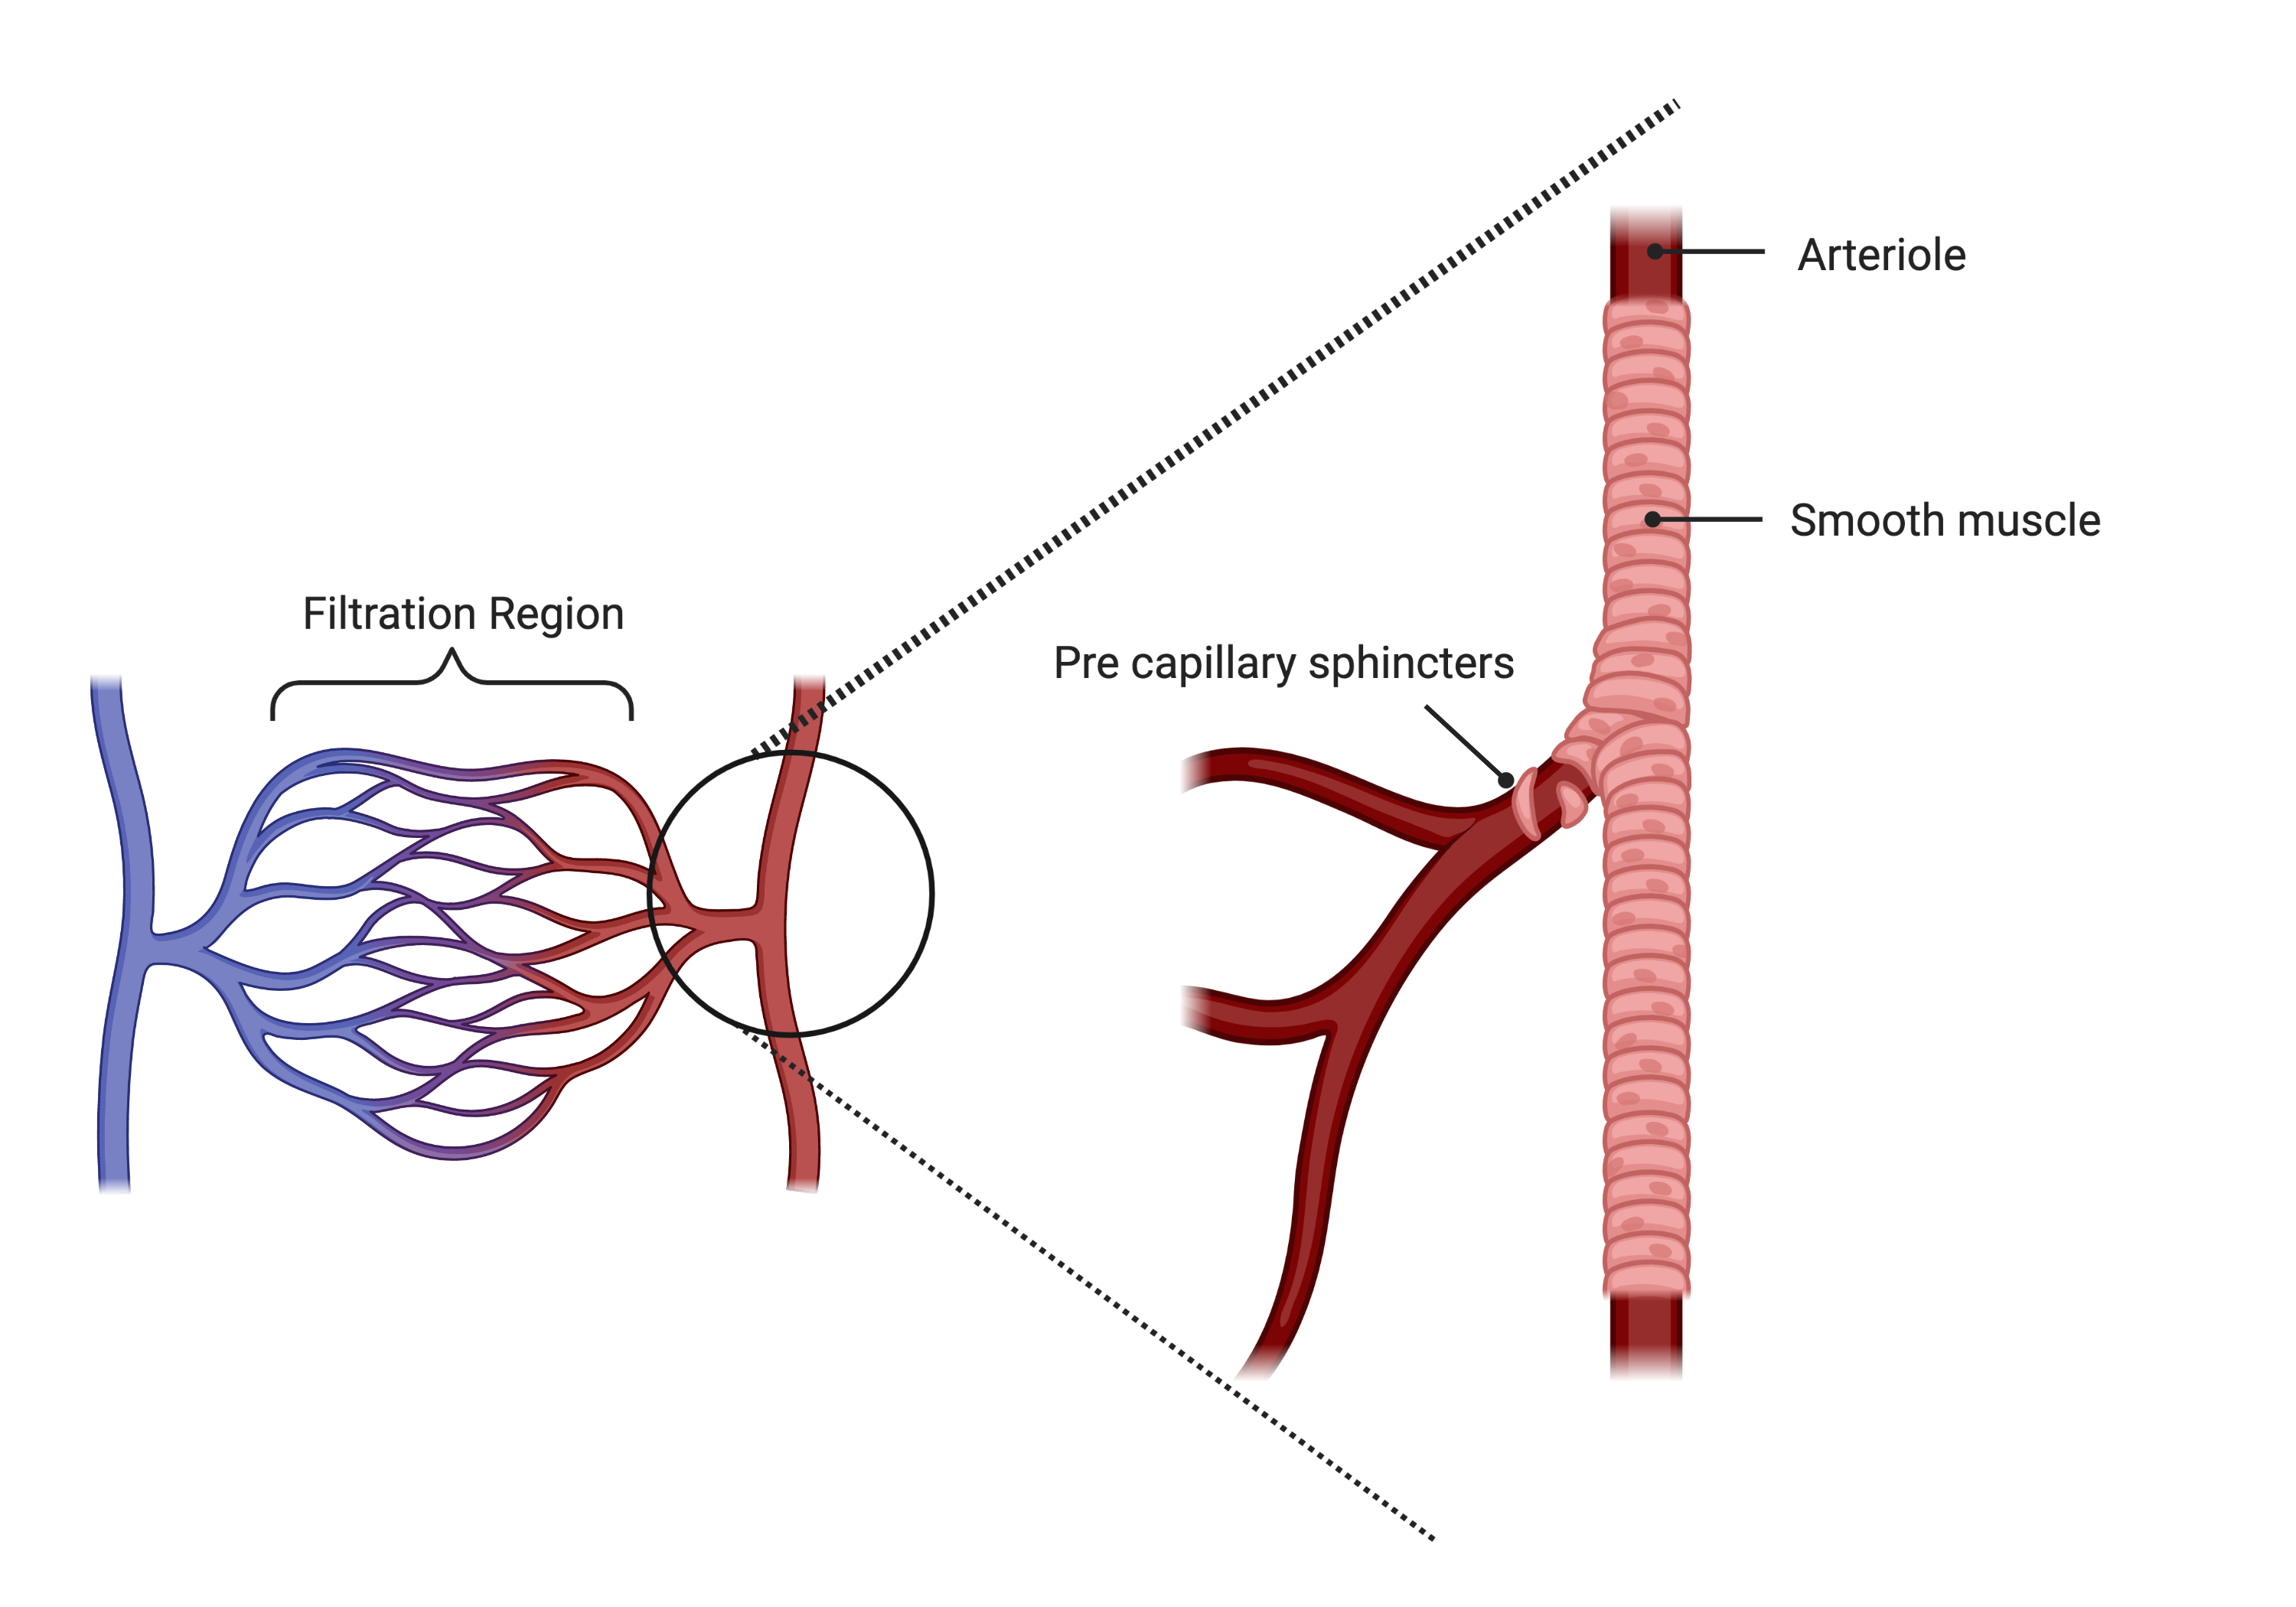
\includegraphics[width=0.7\linewidth]{./figure/capillaries.png}
    \caption{Capillary Anatomy \footnotesize{(Created with BioRender.com)}}
    \label{fig:capillaries}
\end{figure}

\paragraph{Capillary Dilation}
The capillary membrane can also undergo changes to the size of its openings which can allow cells that could not previously leave the vascular compartment to enter the interstitial fluid. When this occurs, such as with capillary dilation in response to cellular inflammatory mediators or other threats to the well being of cells, the white blood cells enter the interstitial space and change the osmolarity and osmotic pressure gradients. It is also possible that a high volume of blood in the capillaries, due to high pressure in the venuoles, will dilate capillaries. In this situation the high hydrostatic pressure tends to be more complicated by a low osmolarity as larger blood proteins of cells are able to leave the vascular compartment.

\subsection{Filtration Pressures}

Filtration is the normal process of exchanging vascular and interstitial fluid (and solute) for micro-circulation. When filtration does not work well there is either hypoxia due to ischemia (not enough $O_2$ being delivered due to no or limited capillary blood flow), extra cellular edema (excessive fluid in the interstitial space), or (rarely) increased blood volume from excessive fluid moving into the vascular space).

To promote normal filtration the overall filtration pressures (hydrostatic (P) and osmotic ($\pi$)) are slightly unbalanced. This unbalance tends toward pushing fluid and solute out of the vascular compartment and into the interstitial compartment, leaving some of the fluid and solute in the interstitial compartment. The volume of fluid and solute left in the interstitial compartment then enters the lymphatic system and reenters the vascular system after circulation and filtration through the lymph vessels and nodes. 

An equation that shows the relationship between the determinants for filtration is depicted in Figure \ref{fig:filtration_equation}. 

\begin{figure}[!h]
    \centering
    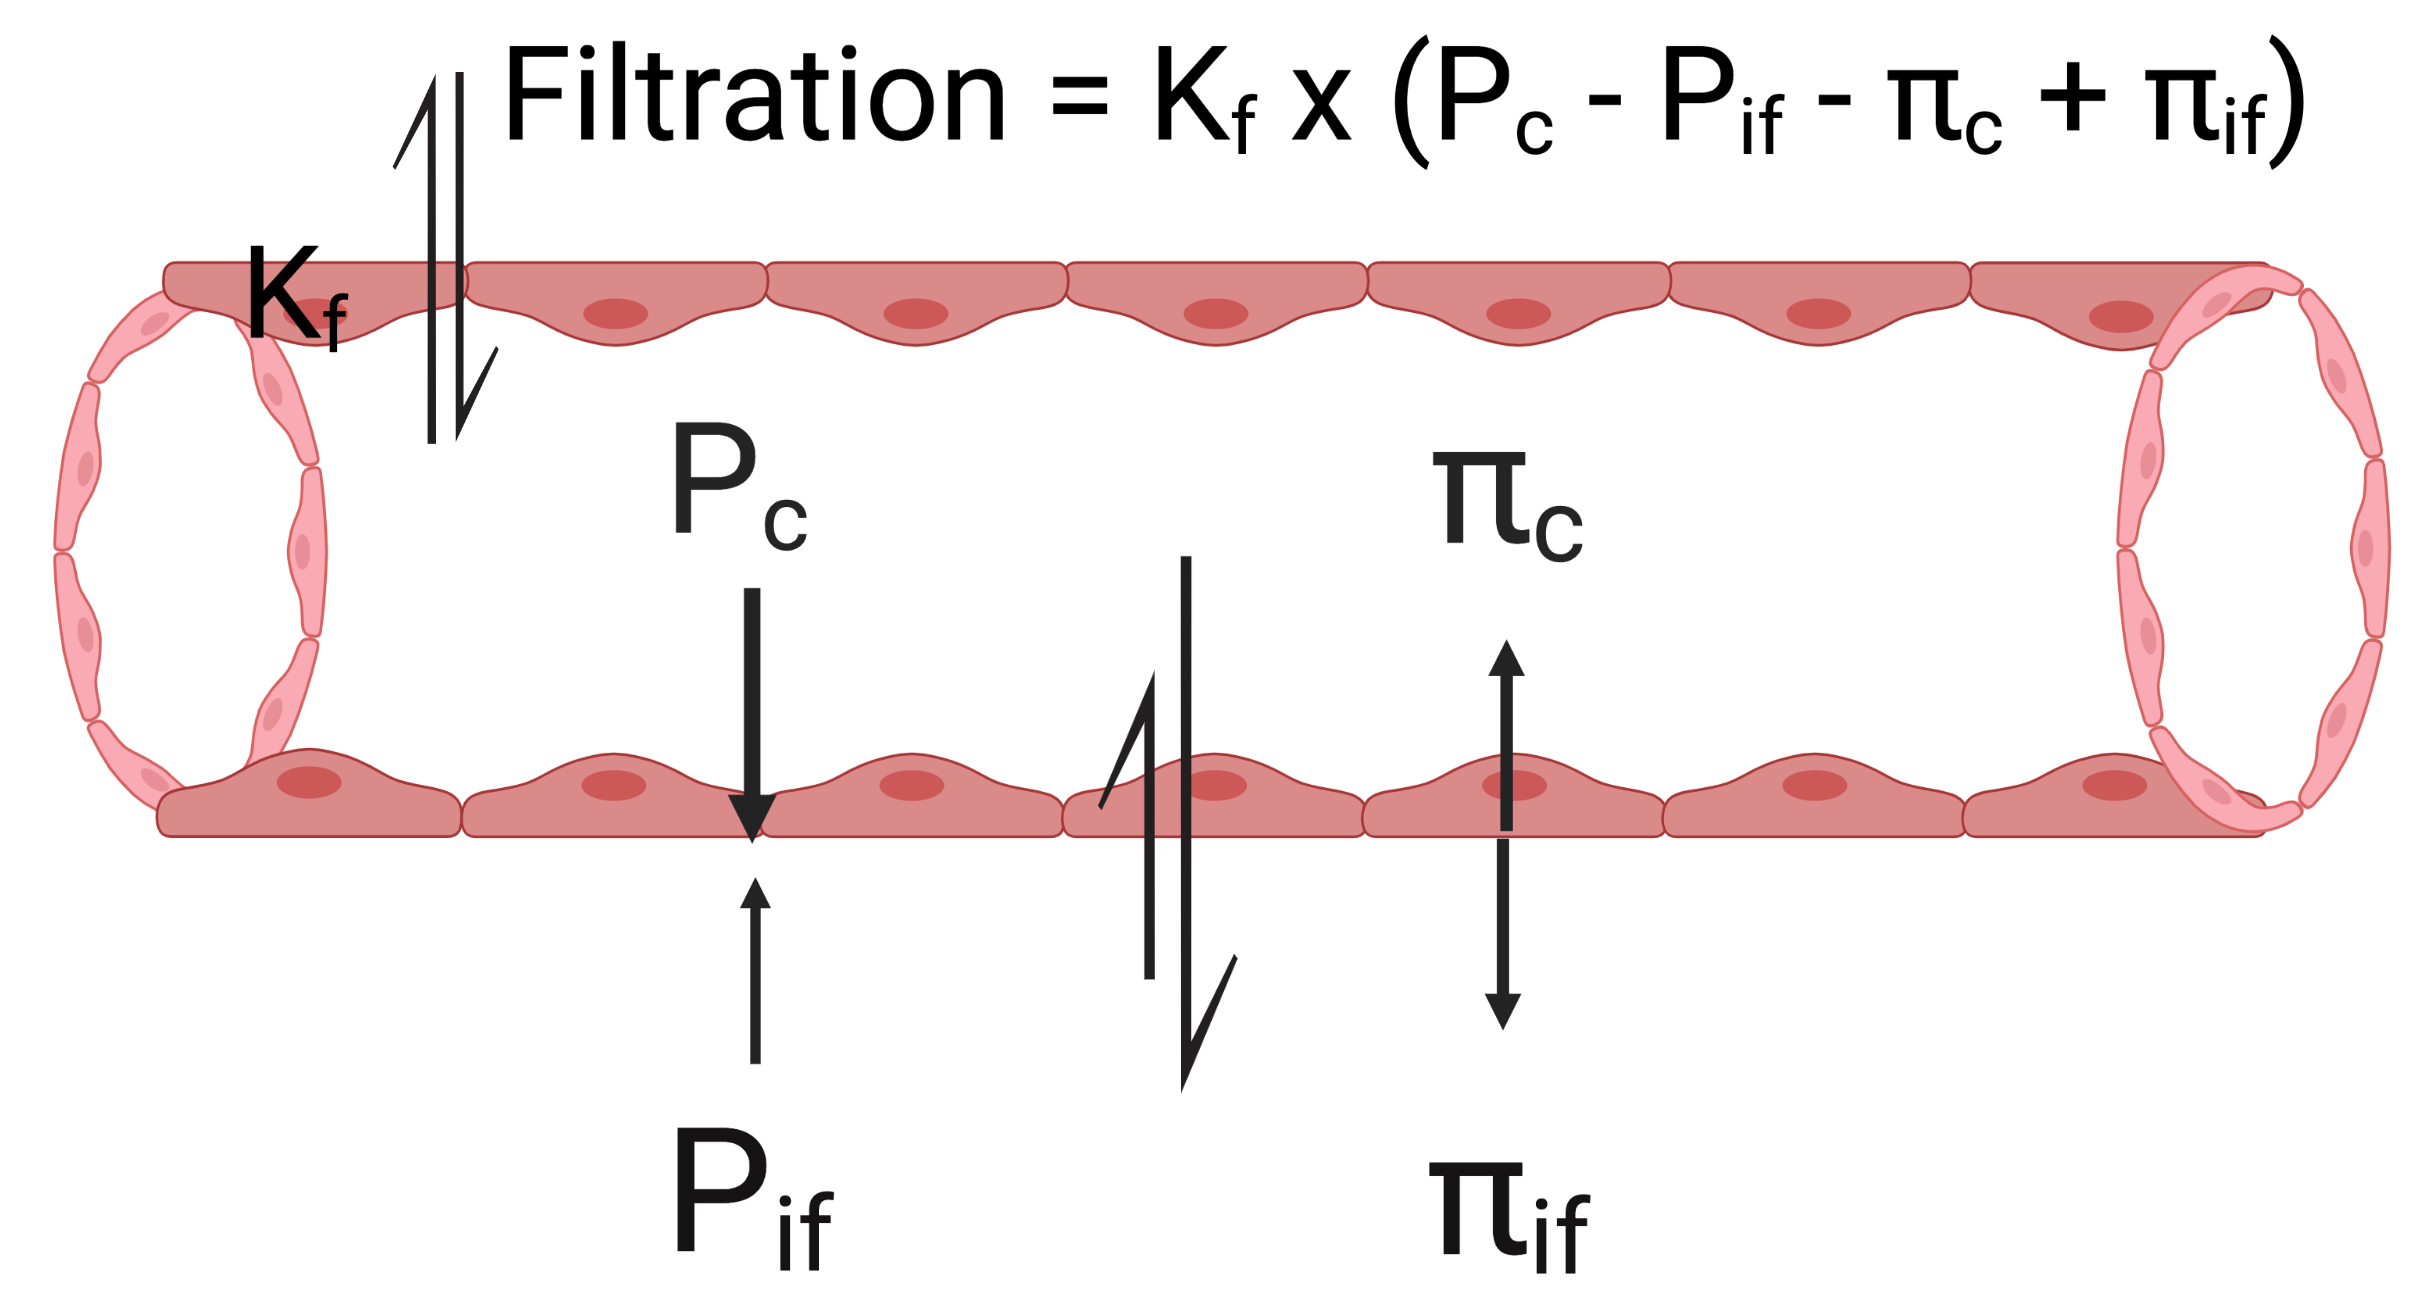
\includegraphics[width=0.7\linewidth]{./figure/filtration_equation.png}
    \caption{Filtration Equation \footnotesize{(Created with BioRender.com)}}
    \label{fig:filtration_equation}
\end{figure}

There are no constants in this equation, each parameter is a variable. The parameter $K_f$ is the filtration coefficient. 

$K_f$ is refers to the permeability of the capillary membrane. While not constant, it is relatively stable unless there are inflammatory mediators caused by injury or infection or very high capillary volumes that cause dilation. Dilation increases the $K_f$ by opening channels between endothelial cells of the capillary membrane. An increase in $K_f$ does not push or pull fluid into a particular compartment. It simply allows more fluid to be moved with any particular balance of filtration pressures.

$P_c$ refers to the hydrostatic pressure inside the capillary, and $P_{if}$ refers to the hydrostatic pressure inside the interstitial fluid (space). The hydrostatic pressures encourage flow from the compartment of higher pressure to lower pressure. $P_c$ pushes solute out of the capillary and into interstitial fluid when it is higher than $P_if$. $P_{if}$ pushes solute out of the interstitial fluid and into the capillary if it is higher than $P_c$.

$\pi_c$ is the osmolarity of the blood in the capillary. It exerts a pressure that pulls water into the capillary (from the interstitial fluid.  $\pi_{if}$ is the osmolarity of the interstitial fluid. It pulls water into the interstitial fluid (from the capillary). 

Since all four of these pressures work with or against one another the overall balance of these four pressures that determines filtration. 

If $(P_c - P_{if} - \pi_c + \pi_{if}) = 0$ there is no net change in vascular or interstitial volume and there would be no filtration. If $(P_c - P_{if} - \pi_c + \pi_{if}) > 0$ there is filtration with a net gain in the interstitial space. If $(P_c - P_{if} - \pi_c + \pi_{if}) < 0$ there is filtration and a net gain in the vascular space. Under normal circumstances, across the entire capillary, $(P_c - P_{if} - \pi_c + \pi_{if})$ is just slightly greater than 0 so that there is filtration and a net gain in the interstitial space that is picked up by the lymphatic system. 

\subsection{Micro-circulation Dynamics Through the Capillary}

The overall process of filtration is a bit more dynamic than depicted in Figure \ref{fig:filtration_equation}. The hydrostatic and osmotic pressures change as blood flows through the capillary, as depicted in Figure \ref{fig:Microcirculation_Regulation}. At the arterial end of the capillary (left side of the Figure) $P_c - \pi_c - P_{if} + \pi_{if} > 0$ which drives solute out of the capillary into the interstitial space. Since the larger items in the blood such as cells and proteins do not move into the interstitial space the $\pi_c$ of the capillary blood increases as the fluid that leaves has a lower osmolarity. Also, as the capillary blood loses volume the the $P_c$ drops. The movement of fluid from the blood into the interstitial space lowers the $\pi_{if}$ and raises the $P_{if}$.

\begin{figure}[!h]
    \centering
    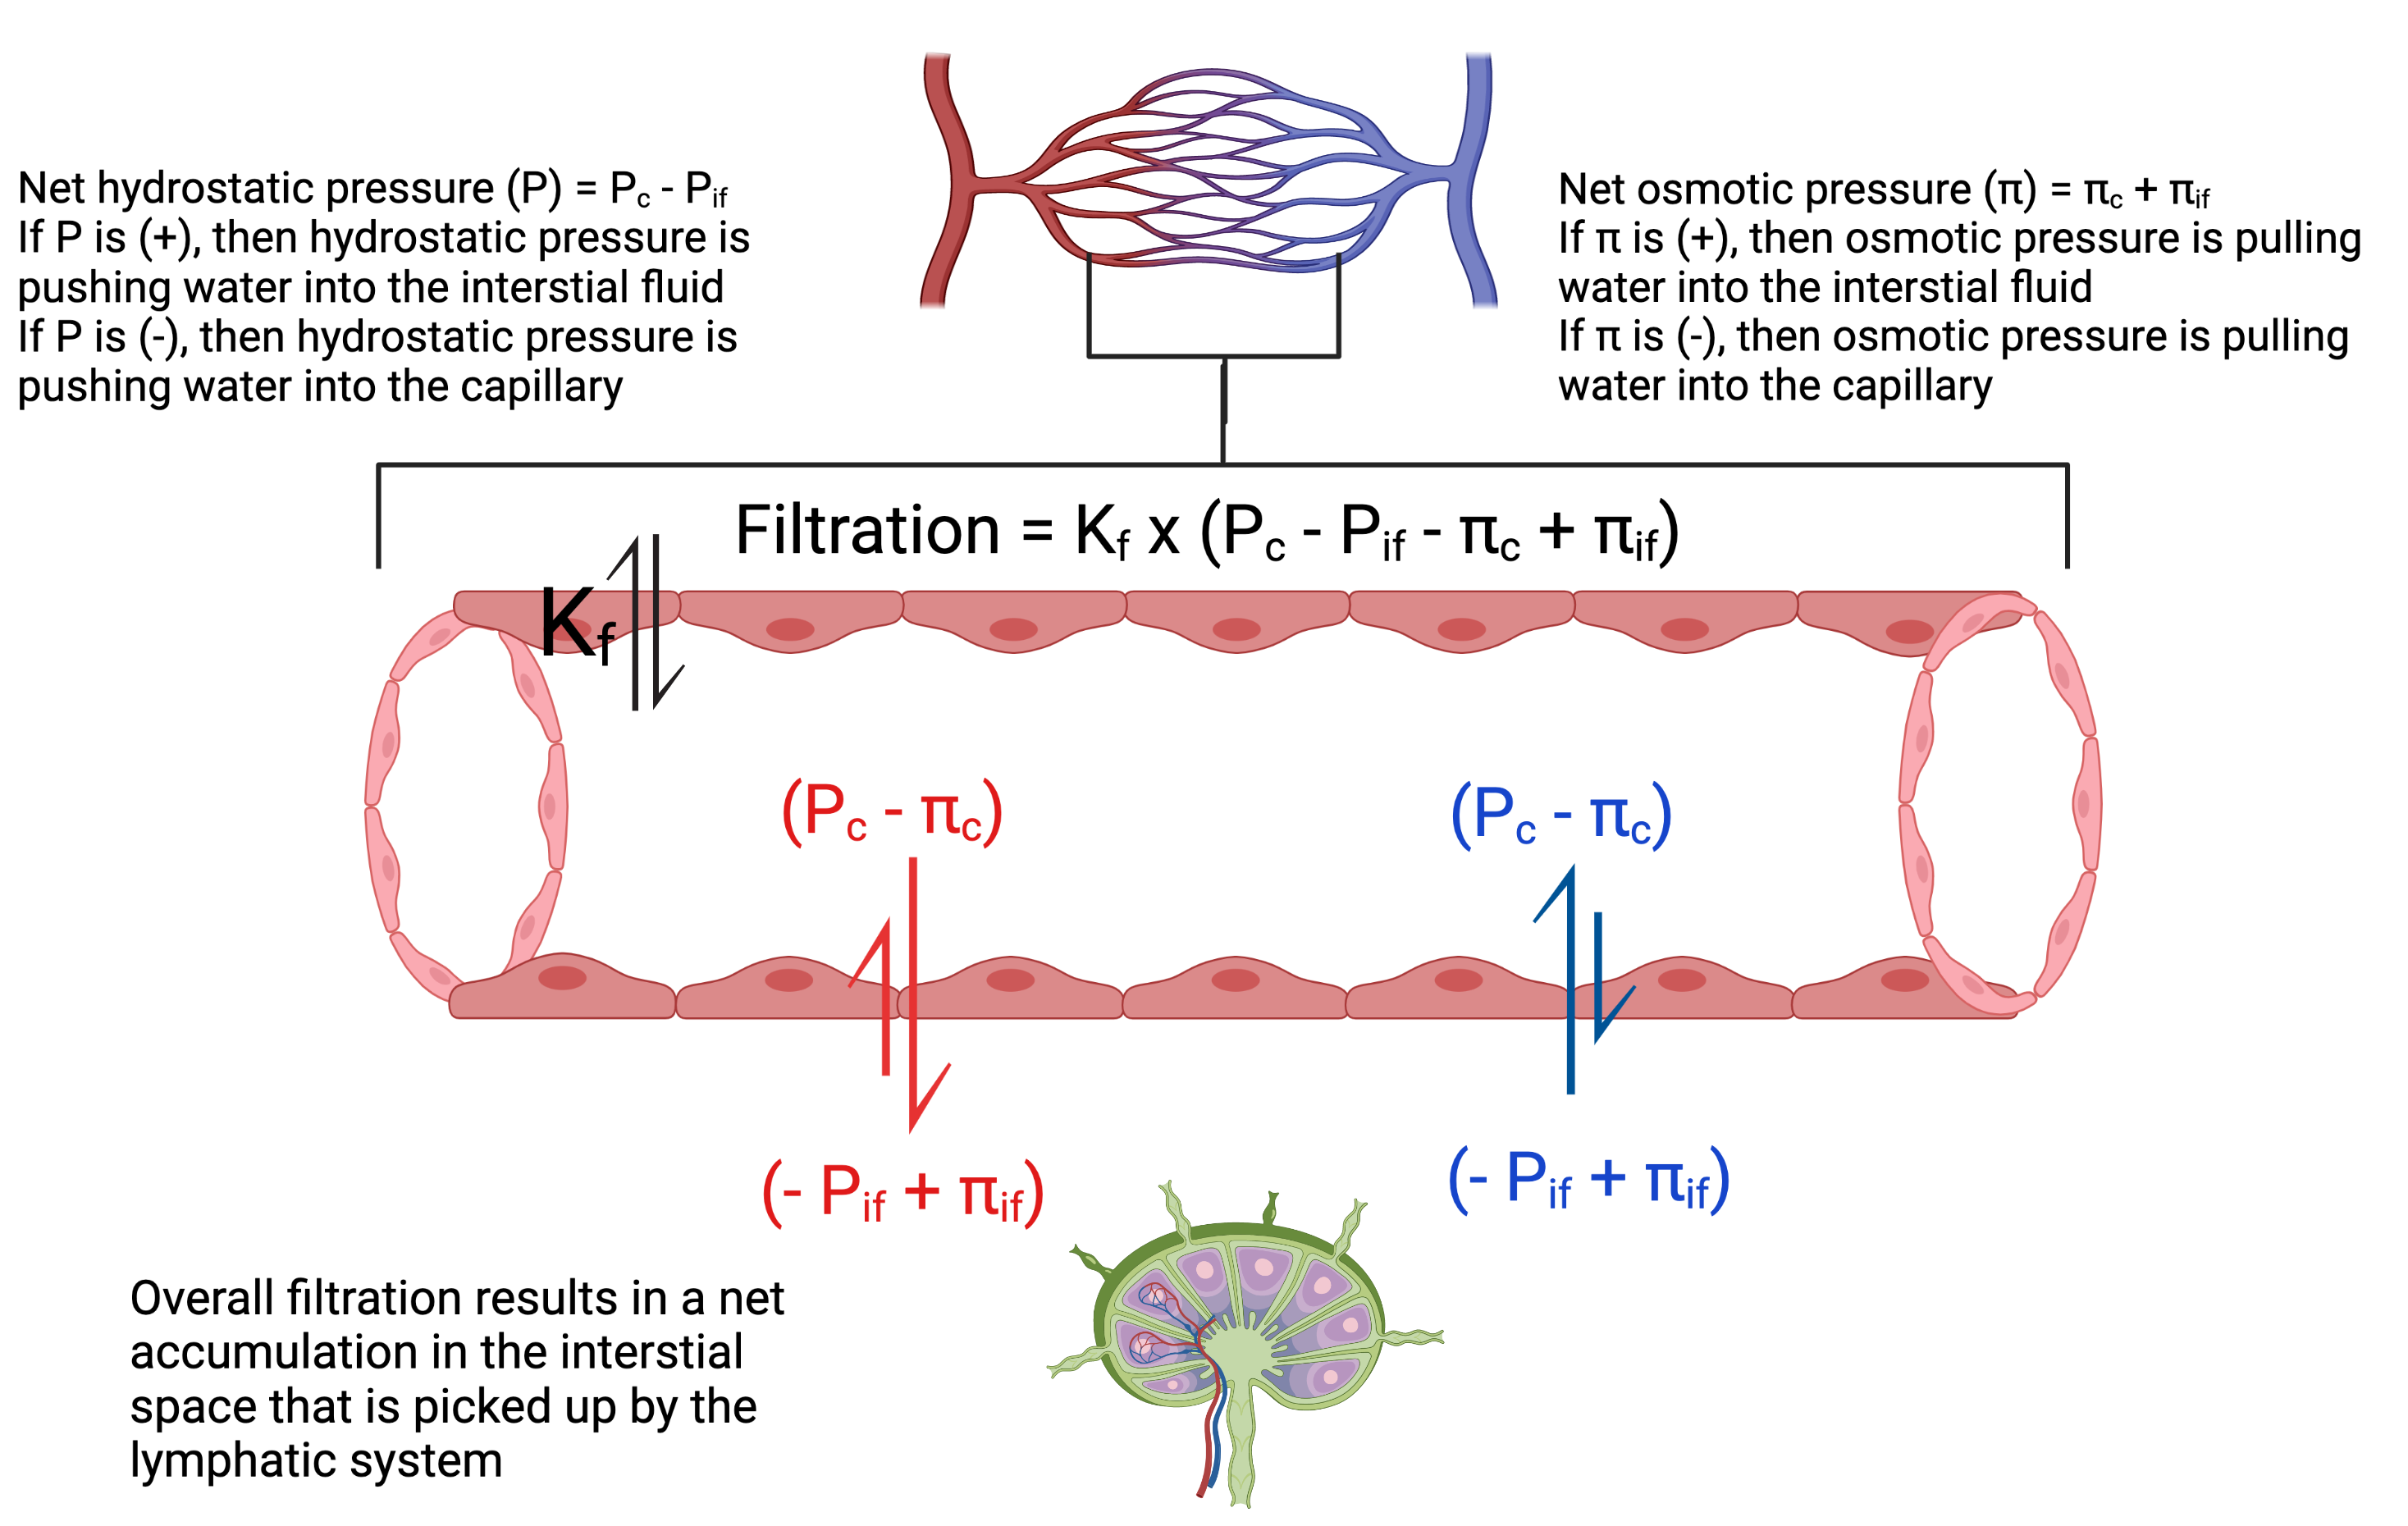
\includegraphics[width=1\linewidth]{./figure/Microcirculation_Regulation.png}
    \caption{Regulation of Micro-Circulation \footnotesize{Created with BioRender.com}}
    \label{fig:Microcirculation_Regulation}
\end{figure}

The overall effect of these changes means that on the venous end of the capillary $P_c - \pi_c - P_{if} + \pi_{if} < 0$ which pulls fluid back into the capillary.  The filtration on the arterial end (fluid pushed out of the capillary) is greater than the filtration on the venous end (fluid pulled into the capillary) so that there is a net positive filtration. This means some of the capillary fluid stays in the interstitial fluid and is picked up the lymphatic system. This more detailed picture of what is happening accounts for the dynamic filtration process going on in capillaries throughout the body. When the fluid on the arterial end of the capillary is pushed out it mixes with interstitial fluid. Then approximately 80\% of fluid is pulled back into the capillary on the venous end. The end result is substantial overall mixing of vascular and interstitial ECF ensuring continuity of ECF throughout the body for homeostasis of ions, delivering nutrients, and removing waste. Additionally, since the remaining 20\% enters the lymphatic system there is a screening process on the plasma passing through the lymphatics which has significant immunological benefits.

\subsection{Factors that Prevent Extra Cellular Edema}

There are a number of situations that result in changes to the overall filtration balance and result in interstitial edema. Some of these situations are minor and self limiting. Mild edema in the lower extremities after a day of being upright (mostly standing) is due to elevated venous pressures increasing $P_c$. There are two safety factors that prevent such situations from becoming severe edema (See Figure \ref{fig:Factors_Prevent_Edema}). First, low tissue compliance limits the hydrostatic pressure gradient as more fluid accumulates in the interstitial space (low compliance means higher pressure with a small change in volume, an increased $P_{if}$). Second, as edema develops there is a decrease in $\pi_{if}$. Third, lymphatic flow can increase by as much as 50-fold. These three factors also interact. As lymphatic flow increases the decrease in interstitial fluid protein further decreases the $\pi_{if}$ concentration in the interstitial fluid reduces the osmotic pressure.

\begin{figure}[!h]
    \centering
    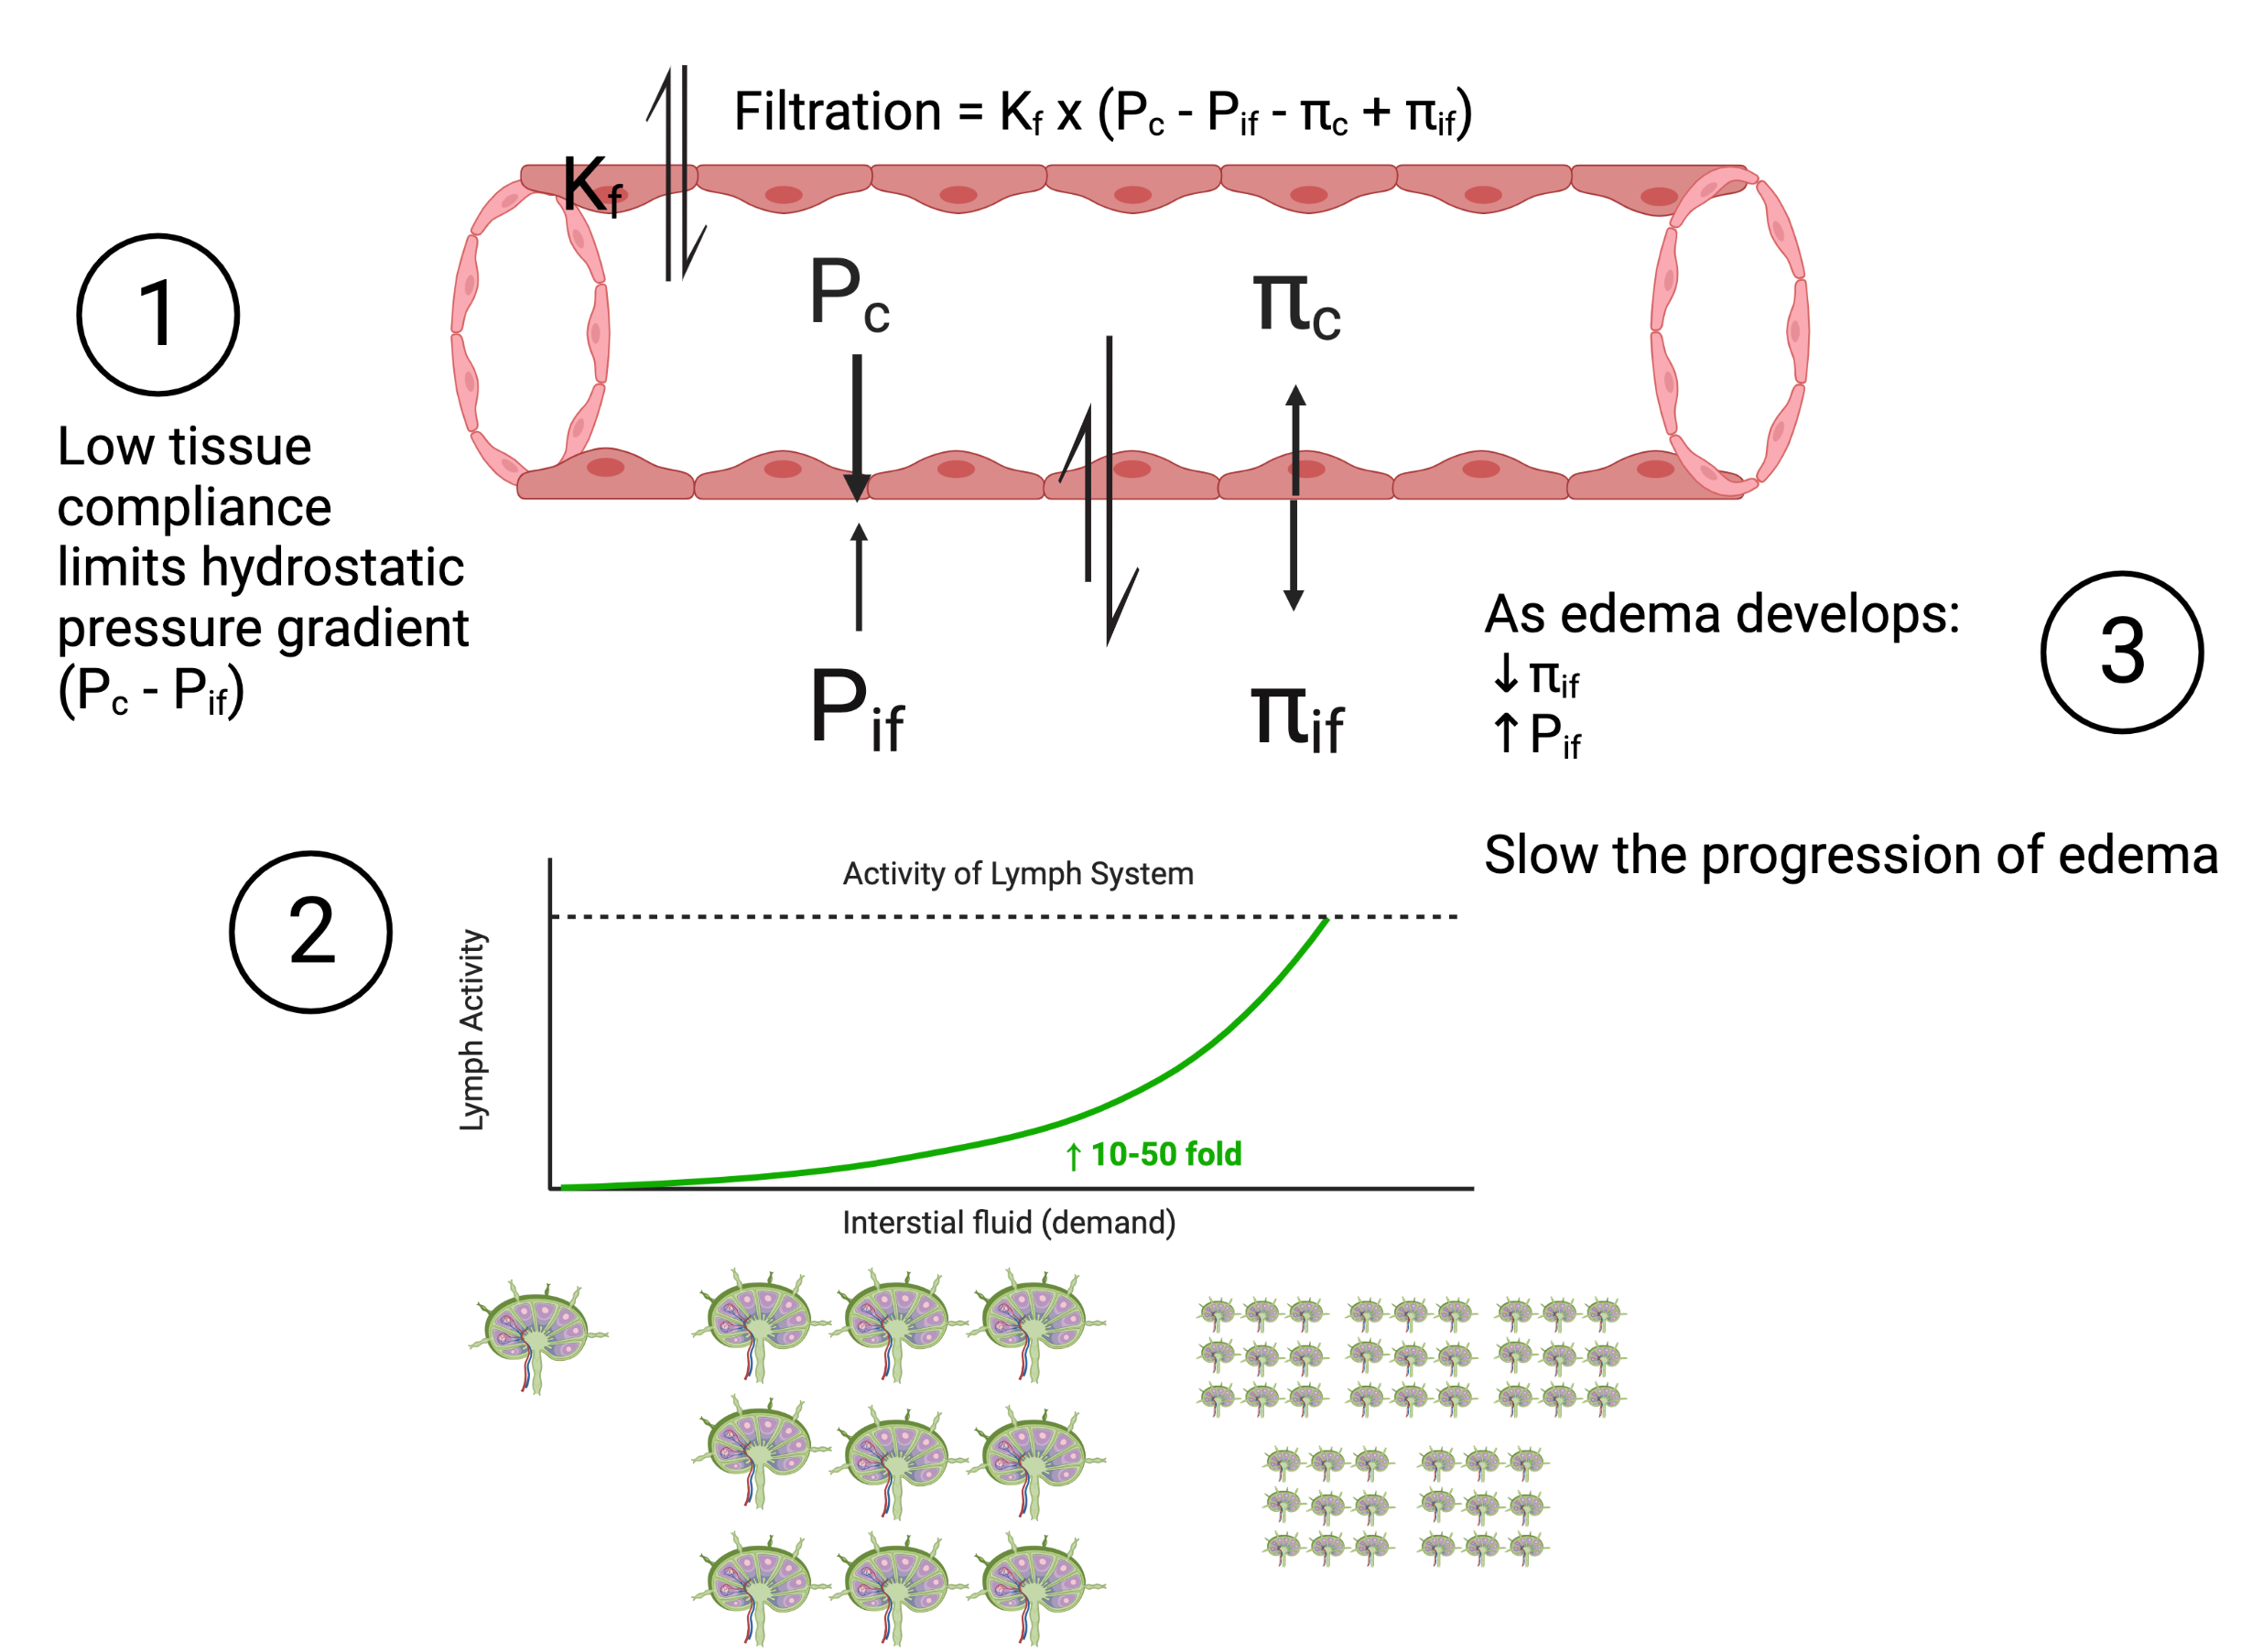
\includegraphics[width=1\linewidth]{./figure/Factors_Prevent_Edema.png}
    \caption{Factors that Prevent Edema \footnotesize{Created with BioRender.com}}
    \label{fig:Factors_Prevent_Edema}
\end{figure}

\subsection{Extra Cellular Edema}

There are two general causes of extracellular edema. First, a higher overall filtration pressure (>> 0) with a greater net flow of solute from the capillary to the interstitial fluid that is not returned to the capillary. This can be caused by anything that increases capillary permeability ($K_f$), alters hydrostatic pressure, or alters osmotic pressure. In these situations the increase in filtration exceeds the capacity of a normal lymphatic system. The problem is caused not by faulty lymphatics, but by an increase in filtration.
The second general cause of extra cellular edema is failure of the lymphatics to pick up extra fluid from the interstitial fluid. In this situation filtration is normal, but the lymphatics are not able to pick up the 20\% of fluid that normal filtration does not return to the capillary. There is a faulty lymphatic system, the edema caused by this situation is called lymphedema.

\begin{figure}[!h]
    \centering
    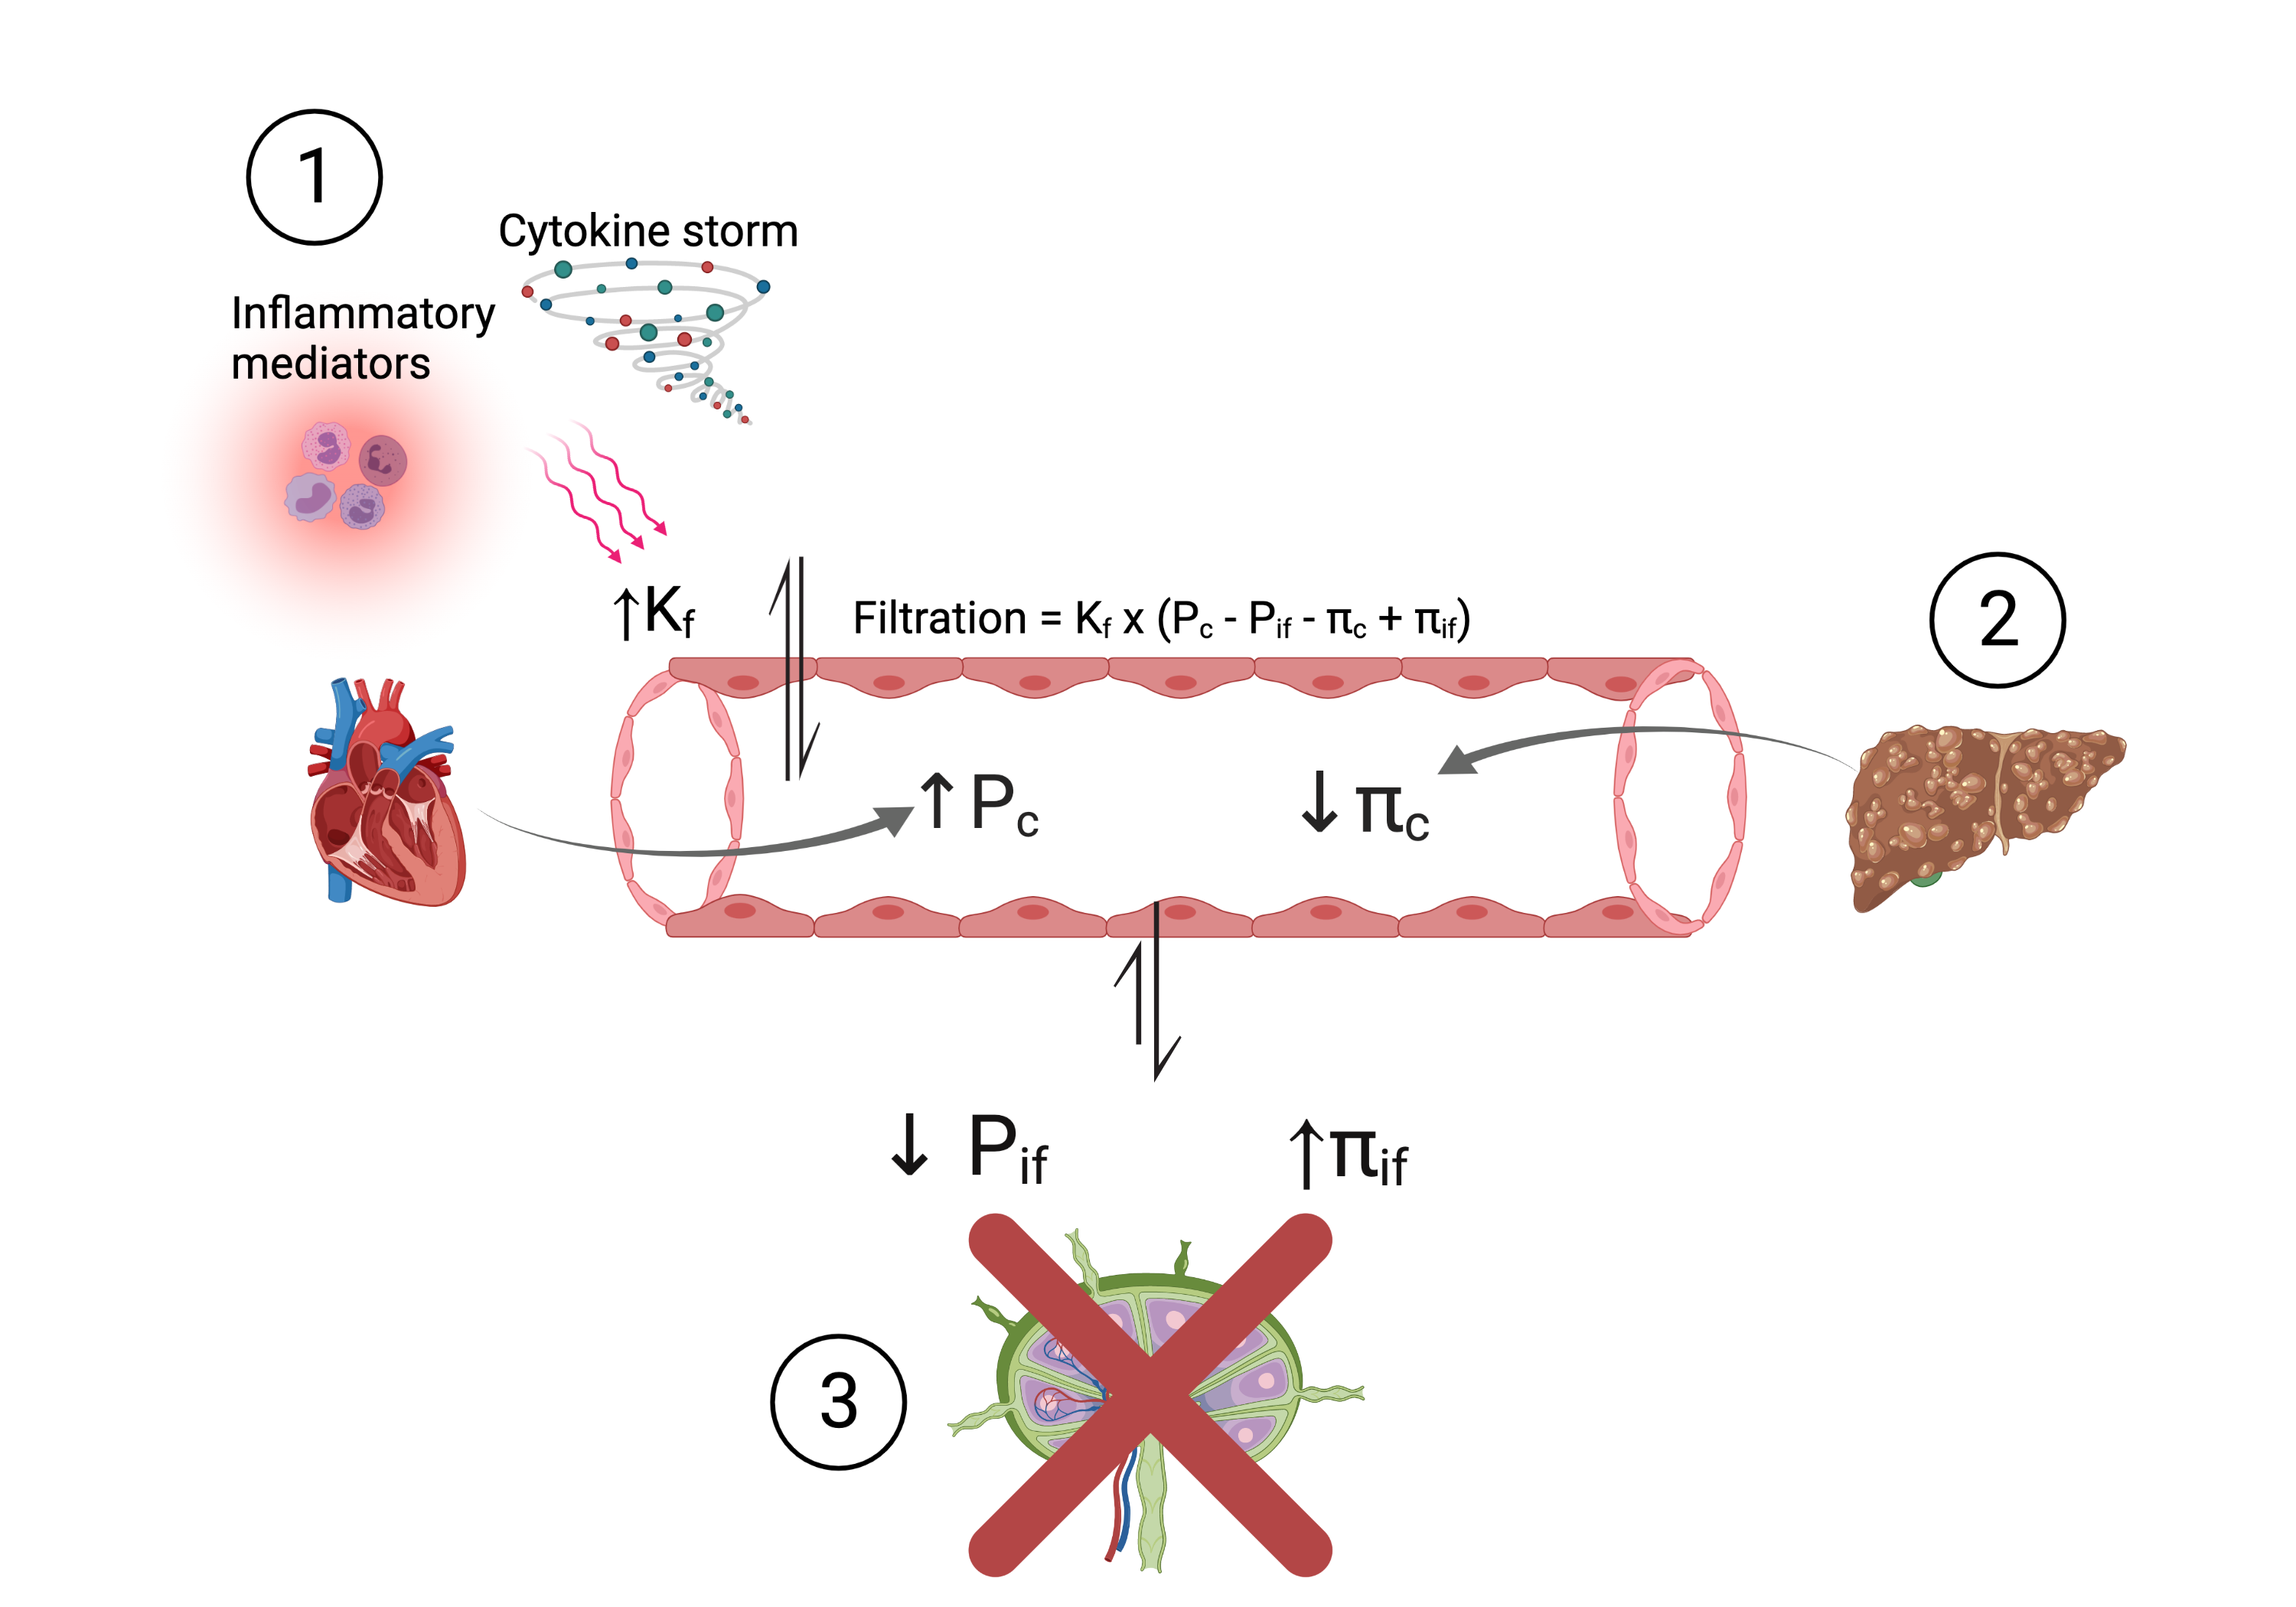
\includegraphics[width=1\linewidth]{./figure/Extracellular_Edema.png}
    \caption{Extra Cellular Edema \footnotesize{Created with BioRender.com}}
    \label{fig:Extracellular_Edema}
\end{figure}

Three particular situations are presented in Figure \ref{fig:Extracellular_Edema} that can cause interstitial edema. Please note that these are not mutually exclusive. 
In situation 1 inflammatory mediators (local damage) or a cytokine storm (systemic inflammation) results in increased $K_f$ which results in a much higher than normal filtration. Since a high $K_f$ can also include movement of larger molecules from the capillaries into the interstitial fluid such as proteins and white blood cells they can have a secondary effect of increasing the $\pi_{if}$ which contributes to the edema. 
In situation 2 there are two examples. To the left, heart failure increases venous pressure due to impaired flow through the heart. The increase in venous pressure increases $P_c$ which pushes more solute out of the capillaries. If this delay in flow is on the left side of heart the edema occurs in the lungs. If it is on the right side of the heart the edema occurs in the extremities (primarily the lower extremities since it is made worse by gravity). It is important to note that the most common cause of a heart pump problem on the right side of the heart is a problem with the left side heart pump. The second example for situation 2 is a reduction in albumin production in liver disease (such as cirrhosis). The reduction in the blood protein albumin reduces $\pi_c$ which lowers the pull of fluid back into the capillaries.
In situation 3 there is failure of the lymphatic flow combined with a lower $P_if$ due to an increase in the compliance of the interstitial space. Without lymphatics removing solute from the interstitial fluid there is also an increase in $\pi_{if}$ despite an increase in fluid.
As with any set of possible comorbidities that are not mutually exclusive (which is most of them), the worst case scenario includes combinations of situations. For example, someone with heart failure and liver disease getting COVID and having a systemic cytokine storm and local inflammatory mediators associated with local hypoxia. 

\section{\textit{Muscle Connections}}

\subsection{Smooth Muscle}

Smooth muscle is present in the walls of organs (i.e. stomach, intestines), passageways (arteries, veins, bronchioles). They are spindle shaped and much shorter than skeletal muscle fibers. Smooth muscles do not have striations but they do have actin and myosin. Unlike skeletal muscles the actin and myosin is not so precisely arranged to form sarcomeres. Fiber arrangement is highly variable between smooth muscles and dependent on the role. 

\paragraph{Smooth Muscle Activation}

Unlike skeletal muscle the tension of smooth muscle fibers acts on other smooth muscle fibers for the purpose of making a compartment or passageway narrow (such as vasoconstriction or vasodilation). Actin is anchored by dense bodies (similar to the Z-discs) which are fastened to the sarcolemma. A smooth muscle contraction is activated by calcium which is supplied by the SR and directly from the  extracellular fluid moving through channels in the smooth muscle sarcolemma. Calcium binds to calmodulin (smooth muscle version of troponin-tropomyosin). When activated the sliding filament theory is similar to skeletal muscle, and the overall effect is tension that attempts, and in most cases does, shorten the fiber. Shortening occurs in most cases because the tension developed does not usually have high resistance preventing the shortening, or at least there are far less variations in the resistances that smooth muscles must compete with (other than perhaps the uterus during labor and delivery where contractions are pushing against a substantial resistance). Since smooth muscle is attached to dense bodies that are attached to the sarcolemma, in addition to shortening smooth muscle tends to also pull inward from all around itself. 

\paragraph{Smooth Muscle Excitation}

Smooth muscle excitation is initiated by the influx of $Ca^{2+}$ which depolarizes the membrane, activates crossbridges and excites SR to release additional $Ca^{2+}$. The wave of excitation over the sarcolemma from fiber to fiber because unlike skeletal muscle when one smooth muscle fiber is activated all should be activated (single-unit organization).

\paragraph{Smooth Muscle Regulation}

Smooth muscles can be organized as a single-unit (more common) or as as a multi-unit.
Single unit smooth muscles have gap junctions that allow quick sharing of $Ca^{2+}$ between cells during excitation so that all the fibers are activated together as a single-unit. Single-unit smooth muscle surrounds the visceral organs and the small blood vessels. Single-unit smooth muscle is regulated by both the autonomic nervous system and stretch. The autonomic nervous system (sympathetic nerves and hormones, parasympathetic nerves) can excite single unit smooth muscles for more or less tension using frequency summation (but not motor unit summation because there are no motor units). Autonomic nerve excitation of single-unit smooth muscle does not occur at precisely located motor end plates and neuromuscular junctions. Instead the autonomic nerves have locations along the nerve fibers called varicosities that are filled with with vesicles that release a neurotransmitter that is then free to bind to any acceptable and available smooth muscle receptor (See Figure \ref{fig:Smooth_Muscle}). Single-unit smooth muscle also can be excited by stretch in what could be considered a local stretch reflex. Unlike a muscle spindle stretch reflex in skeletal muscle that loops through the spinal cord, the smooth muscle stretch reflex occurs because the mechanical stretch of the fiber opens $Ca^{2+}$ channels that both excite and activate the smooth muscle.

\begin{figure}[!h]
    \centering
    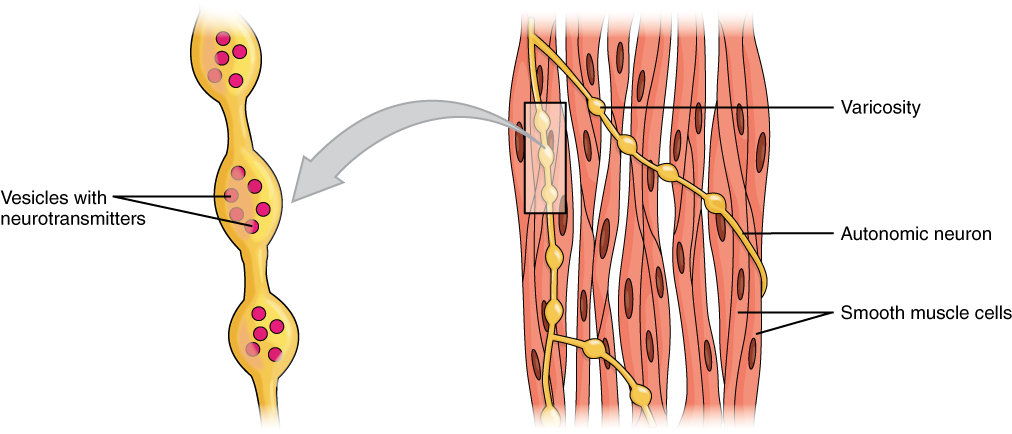
\includegraphics[width=0.5\linewidth]{./figure/Smooth_Muscle.jpg}
    \caption{Smooth Muscle \footnotesize{CCBY4.0 from Version 8.25 from the Textbook OpenStax Anatomy and Physiology}}
    \label{fig:Smooth_Muscle}
\end{figure}

Multi-unit smooth muscle fibers can be regulated by both frequency and fiber unit based excitation. To allow this increase in precision of tension for multi-unit smooth muscles they have precision between the autonomic nerves and the smooth muscle fibers. They also do not have gap junctions so excitation does not spread from one fiber to the next. Like skeletal muscle, excitation is confined to the fiber that was originally excited. Excitation for multi-unit smooth muscles also does not originate from stretching. The large blood vessels and the respiratory airways have multi-unit smooth muscle.

\paragraph{Smooth Muscle Tone}

Activation continues until ATP-dependent calcium pumps actively transport $Ca^{2+}$  ions back into the SR and out of the cell. Many smooth muscles maintain a low concentration of  $Ca^{2+}$ to maintain tone. In the case of blood vessels this is important because if all blood vessels were fully dilated (no smooth muscle tone) then blood pressure would drop so low that maintaining upright posture would not be possible. Abnormalities in the smooth muscle tone of blood vessels one possible cause for conditions such as orthostatic hypotension, postural orthostatic tachycardia syndrome (POTS) and vasovagal syncope.

To allow smooth muscles to maintain tone for prolonged periods without rest they can maintain contractions even as  $Ca^{2+}$ is removed and myosin is inactivated. This can happen due to a subset of crossbridges form latch-bridges. Latch bridges keep actin and myosin connected without ATP, allowing tension (as tone) in smooth muscle that lines arterioles and other visceral organs with very little energy expenditure.

\subsection{Compression}

Compression is an important part of edema management (RICE stands for rest, ice, compression and elevation). Elevation reduces hydrostatic pressure. Compression increases the gradient between venous pressure being compressed and venous pressure further away from compression (usually more proximal). This encourages reduction in $P_c$ which allows more fluid to reenter the capillary during filtration. The pressure also increases the pressure gradient between the local lymphatics and the lymph vessels not being compressed which facilitates movement of edema also into the lymphatics.

Compression has also now become more common for recovery to increase micro circulation to remove post exertion waste and delivery needed nutrients. It works through the same mechanisms as above, but in response to small amounts of local edema from a combination of increased cellular and interstitial osmolarity, and increased cellular and capillary permeability ($K_f$). The compression does not alter the permeability, or the osmolarity changes, but it does reduce $P_c$ which shifts the balance of the filtration equation to encourage movement of edema from the area and into both the capillary and lymphatics.

Compression is also gaining popularity during endurance events, particularly running. However whether there is a benefit and what the mechanisms are remains elusive \cite{mota_effects_2020}. There are several factors to consider with compression during endurance events and it goes beyond what can be discussed in this already long chapter. On reason proposed for compression during an endurance event is to maintain vascular volume. With such long events may be difficult to maintain complete hydration. However, a small amount of dehydration increases $\pi_c$ which facilitates return of fluid into the circulation. There is also a strong muscle pump working to maintain venous flood flow, once again, facilitating return of fluid to the capillary (keeps $P_c$ low due to venous blood flow and would also promote lymphatic blood flow). So it is unclear whether sustaining vascular volume makes mechanistic sense. It's possible that it facilitates greater overall micro circulation and filtration which encourages greater nutrient delivery and waste product removal from the lower extremities. It is also quite possible that whether compression with endurance running provides a benefit is highly contextual (i.e. related to many interacting causal factors, complex) and is difficult to completely account for in research studies. In such situations it may be best trialed by individuals with self experimentation, which requires a slight reconsideration of what it means to gather evidence \cite{anjum2020rethinking}.

\section{Summary}

The ECF supports muscle fibers by having and providing resources for muscle function. ECF requires micro-circulation. Micro-circulation between cells and the ECF requires balanced osmolarity and a functioning semi-permeable sarcolemma (cell membrane). Micro-circulation between the compartments of ECF, vascular (capillary) and interstitial spaces (fluids) requires filtration. Filtration requires a small unbalance of hydrostatic and osmotic pressures between the capillaries and the interstitial spaces as well as a semi-permeable capillary membrane. Water, ions, molecules and nutrients are constantly circulating between the vascular (capillaries and lymphatics) and interstitial compartments of the ECF. 
The amount of blood flowing through capillaries can be varied by local and neuroendocrine factors by altering the degree of vasodilation and vasconstriction of arterioles, pre-capillary sphincters and venuoles. Vasoconstriction occurs through tone (sustained contraction) of smooth muscles. 
All causes of intra cellular and extra cellular can ultimately be broken down into altered membrane permeability (cell or capillary), imbalances of osmolarity (and osmotic pressure), imbalances of hydrostatic pressure, and lymphatic function. Compression is an effective intervention for edema due to its facilitation of venous blood flow which reduces $P_c$.


\section{Next Steps}

The next chapter is on blood flow (circulation), the flow of blood through the entire circulatory system. Circulation of blood through the entire body ensures regular mixing of the ECF contents throughout the body. This mixing ensures consistency of ECF contents and a stable environment for all the cells of the body. Circulation allows each supporting system to contribute by either to adding to ECF or removing by-products from ECF. Circulation also allows supporting systems to communicate with each other based on the circulating substances and messages (hormones). Blood flow requires a pump (the heart), vessels from the heart to the capillaries (arteries) and from the capillaries back to the heart.

\printbibliography[heading=subbibintoc]
